\section{Numerical Experiments}\label{sec:numexp}
%
We now use \Cref{alg:refSeries} to solve goal-oriented inverse problems in a multi-model setting; the method used to localize the error estimate is described in \Cref{sec:errLocal}. We first consider two-dimensional models in order to explore the behavior of the algorithm as well as the effect of varying the placement of observations and QoI regions. In \Cref{sec:cdvcdr}, the high-fidelity model is a convection-diffusion-reaction nonlinear model, and the low-fidelity model is a linear convection-diffusion model. We apply \Cref{alg:refSeries} to this pair of models, and then examine how the localized error estimate is affected by changes in sensor placement and in the QoI region. In \Cref{sec:constvfield}, both the high- and low-fidelity models are convection-diffusion-reaction nonlinear models, but they differ in how the parameter is represented. In \Cref{sec:diffvcdr3D}, we consider a more realistic pair of three-dimensional models, again targeting a convection-diffusion-reaction problem.

%In all experiments, starting the simulation with the low fidelity model, we seek to add regions of high fidelity, until the estimated relative error in the target QoI is less than 1$\%$.

%------------------------------------------------------------------------------------------------------------------------%
\subsection{Variable Physics: Convection-Diffusion(-Reaction)} \label{sec:cdvcdr}
%------------------------------------------------------------------------------------------------------------------------%
In this section, we consider a pair of models which differ in the physics included. In \Cref{sec:cdvcdrSetup} we describe a baseline setup for a simple two-dimensional problem. \Cref{sec:cdvcdrBaseRef} describes the results of applying \Cref{alg:refSeries} to the baseline problem, and \Cref{sec:qoivdata} describes the results of changing the placement of the observations or the QoI region from the baseline.
%
%------------------------------------------------------------%
\subsubsection{Problem Setup} \label{sec:cdvcdrSetup}
%------------------------------------------------------------%
%
We consider a rectangular domain $\Omega(x_1,x_2)=[0,5]\times[0,1]$, where $x_1$ and $x_2$ are the spatial coordinates. The high-fidelity model is a single-species convection-diffusion-reaction equation with a nonlinear reaction term, described by,
%
\begin{subequations}
\label{eq:cdvcdrHF}
\begin{align}
k_d\nabla^2 u - \vec{V}\cdot\nabla u + k_ru^2 = f(q) \quad &\text{in } \Omega, \label{eq:cdvcdrHF_int} \\
u = 0 \quad &\text{on } \partial \Omega, \label{eq:cdvcdrHF_bdry}
\end{align}
\end{subequations}
%
where the state $u$ is the species concentration and $f(q)$ is a forcing field described by the parameters. We have a divergence-free parabolic-profile velocity field $\vec{V}(x_1,x_2) = (2x_2(1-x_2),0)$; the diffusion and reaction coefficients are $k_d = 0.1$ and $k_r = -42.0$, respectively. The low-fidelity model,
%
\begin{equation}
k_d\nabla^2 u - \vec{V}\cdot\nabla u = f(q)
\end{equation}
%
differs only in the removal of the reaction term. To form the mixed-fidelity models, we divide the domain into complementary subdomains, $\Omega_{HF}$ and $\Omega_{LF}$, where the high- and low-fidelity models are solved, respectively. The resulting mixed-fidelity models can be described by,
%
\begin{equation}
k_d\nabla^2 u - \vec{V}\cdot\nabla u + k^{MF}_ru^2= f(q),
\end{equation}
%
where $k^{MF}_r$ is a piecewise-constant reaction coefficient,
%
\begin{equation}
k^{MF}_r=
\begin{cases}
k_r & \textrm{if }x\in\Omega_{HF} \\
0 & \textrm{if }x\in\Omega_{LF}.
\end{cases}
\end{equation}
%
Homogeneous Dirichlet boundary conditions are applied on the entire boundary of the domain. The QoI we wish to calculate is the integral of the state,
%
\begin{equation}
I(q,u)=\int_{(x_1,x_2)\in \Omega_I} u \:\textrm{d}A,
\end{equation}
%
over a region $\Omega_I=[0.625,0.875]\times[0.375,0.625]$.

The unknown parameters to be inferred correspond to the forcing field, so that in this case $f(q)=q$. The observations are sparse measurements of the state.
\Cref{fig:baseSetup} shows the locations of the observations and the region $\Omega_I$ over which the QoI is calculated. For the low-fidelity model, the inverse problem is linear (i.e., the observations depend linearly on the parameters). Since the inverse problem is ill-posed, we use Tikhonov regularization~\cite{EngHanNeu00}; the regularization term in the objective function \Cref{eq:invOpt_obj} is $R(q)=\frac{\beta}{2}\int_\Omega \|\nabla f(q)\|_2^2\:\textrm{d}A$, where $\beta=10^{-5}$ is the regularization coefficient.
%
\begin{figure}[htbp]
\centering
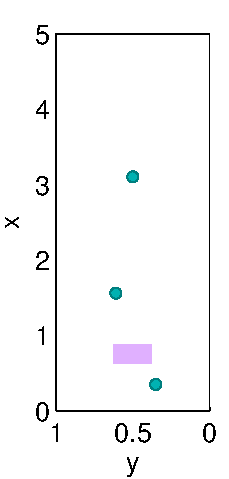
\includegraphics[width=0.8\textwidth]{baseSeries/setup_3_3.pdf}
\caption{Locations of the observations and the QoI region.}
\label{fig:baseSetup}
\end{figure}
%

For the numerical simulations, we use the finite element method (FEM), employing a continuous Galerkin formulation with Lagrange elements. We use the \texttt{libMesh} library~\cite{libMeshPaper} for the FEM calculations.
%\red{The library offers easy calculation of adjoint systems, error estimates and subdomain restricted variables.}\footnote{But we don't use Libmesh's error estimates or restrict variables to subdomains...}
The domain is discretized by a regular mesh of quadrilaterals, with 250 and 50 elements along the $x_1$ and $x_2$ directions, respectively, for a total of 12,500 elements, resulting in 12,801 degrees of freedom per variable. The diffusion coefficient is such that the cell P\'{e}clet number never exceeds 0.1, and thus no stabilization is required.

Synthetic observations consisting of the state at three points in the domain are artificially generated by running the high-fidelity model on a finer mesh with the true forcing field
%
\begin{equation}
f_{true}(x_1,x_2)=
\begin{cases}
1.0 & \textrm{if }(x_1,x_2)\in[0.125,0.375]\times[0.125,0.375] \\
0.8 & \textrm{if }(x_1,x_2)\in[2.375,2.625]\times[0.375,0.625] \\
0 & \textrm{otherwise}.
\end{cases}
\end{equation}
%
%
%------------------------------------------------------------%
\subsubsection{Adaptive Model Refinement Results} \label{sec:cdvcdrBaseRef}
%------------------------------------------------------------%
%

We now present the results for solving the inference problem using \Cref{alg:refSeries}. Once the QoI error estimate is calculated using \Cref{eq:finErrExp}, the error estimate is then decomposed into local contributions. At each iteration, based on this decomposition, we choose the basis functions with the largest error contributions until an additional 5\% of the elements has been marked for refinement. This is repeated until the estimated absolute relative error in the QoI, calculated as $\epsilon_i/(\epsilon_i+I(q_{MF_i},u_{MF_i}))$, is less than $1\%$.

\Cref{fig:baseRef} shows the local error contributions, as well as the subdomains where the low- and high-fidelity models are used, for the series of mixed-fidelity models thus generated. %Each linear Lagrange basis function's contribution is plotted at its nonzero node.
%
\begin{figure}[htbp]
%\captionsetup[subfloat]{captionskip=-5pt}
\centering
\subfloat[LF $\equiv$ MF$_0$ ($0\%$ HF)]{
  \includegraphics[width=0.46\textwidth]{baseSeries/cd_cdr_LF_divvy.png}
  \includegraphics[width=0.49\textwidth]{baseSeries/err_breakdown_LF.png}
  \label{fig:baseRef0}
} \\
\subfloat[MF$_1$ ($5\%$ HF)]{
  \includegraphics[width=0.46\textwidth]{baseSeries/cd_cdr_MF01_divvy.png}
  \includegraphics[width=0.49\textwidth]{baseSeries/err_breakdown_MF01.png}
} \\
\subfloat[MF$_2$ ($10\%$ HF)]{
  \includegraphics[width=0.46\textwidth]{baseSeries/cd_cdr_MF02_divvy.png}
  \includegraphics[width=0.49\textwidth]{baseSeries/err_breakdown_MF02.png}
} \\
\caption{Left: Multi-fidelity refinement over the domain (low-fidelity convection-diffusion model used in red portion, high-fidelity convection-diffusion-reaction model used in blue portion). Right: local error contributions. }
\label{fig:baseRef}
\end{figure}
%
Note that the error contribution of each basis function whose support is entirely within the high-fidelity regions is zero.

We see that the largest local error contributions are concentrated in the QoI region and around the observation location closest to the QoI. In the first decomposition of the error (\Cref{fig:baseRef0}), the region where the elemental error is greatest is around the leftmost observation location. Since the constraining model is an elliptic PDE, with weak convection, information flow is localized, and is weakly convected from left to right. Therefore, for the calculation of the QoI, it is most important to refine the region near the leftmost observation location, and then around the QoI region. After that, the error decomposition suggests refinement in regions upstream and around the middle observation location, and then the rightmost observation location.

\Cref{fig:baseErr} shows the true and estimated absolute relative errors in the QoI for the various mixed-fidelity models generated by \Cref{alg:refSeries}; the true and estimated relative errors are calculated relative to the true and estimated high-fidelity QoI, respectively. In this case, we see that QoI error of $1\%$ is attained with a mixed-fidelity model where the high-fidelity model is used in only about $10\%$ of the domain. We note that while here the error is seen to decrease with increasing refinement, in general there is no guarantee that either the error in the QoI or the relative error in the error estimate will decrease monotonically as more of the domain is refined.
%
\begin{figure}[htbp]
\centering
\includegraphics[width=0.8\textwidth]{baseSeries/err_est.pdf}
\caption{True and estimated absolute relative error in QoI, plotted as a function of the percentage area of the domain in which the high-fidelity convection-diffusion-reaction model is used.}
\label{fig:baseErr}
\end{figure}
%

%------------------------------------------------------------%
\subsubsection{Interaction of Observations and QoI} \label{sec:qoivdata}
%------------------------------------------------------------%
%
The error estimate decomposition suggests the use of the high-fidelity model in areas of the domain that are important to the interaction between the observations and QoI; the interaction between these two can be complex, and the areas suggested for refinement may be nonintuitive. To see this, we compare the error estimate decomposition for three sizes of the QoI region $\Omega_I$ given the same set of observation locations, and for three nested sets of observation locations given the same QoI region. For the sake of illustration, we make two refinement iterations for each combination of observations and QoI region, regardless of the magnitude of the relative error estimate. However, in conducting the numerical experiments, it was observed that the number of iterations needed to achieve a given tolerance tended to increase as the QoI region increased.

\Cref{fig:qoiStudy} shows the domain for three cases considered, with the same set of observations but increasingly large, nested QoI regions $\Omega_I$.
The error decompositions for each case are also shown in \Cref{fig:qoiStudy}. The bottom row gives the baseline case presented in \Cref{sec:cdvcdrBaseRef}, although here we choose the basis functions $i$ whose error $\varepsilon_i$ are among the largest $5\%$, rather than only enough basis functions to cover 5\% of the domain in their support, so the proportion of elements marked for refinement in each iteration will be slightly larger than in \Cref{sec:cdvcdrBaseRef}.
% KW: I don't understand this last sentence. What's the difference with Section 4.1.2?
Although refinement is still most important around the observation location closest to $x_1=0$, as the QoI region expands the other two observation locations become more important in that the error decomposition suggests refinement around them earlier. As the QoI region expands, it is also more clearly noticeable that refinement is not equally important in all parts of the QoI region.

\begin{figure}[htbp]
\centering
\captionsetup{justification=centering}
\subfloat[Locations of observations and QoI region $\Omega_I$][Locations of \\observations and \\QoI region $\Omega_I$]{
  %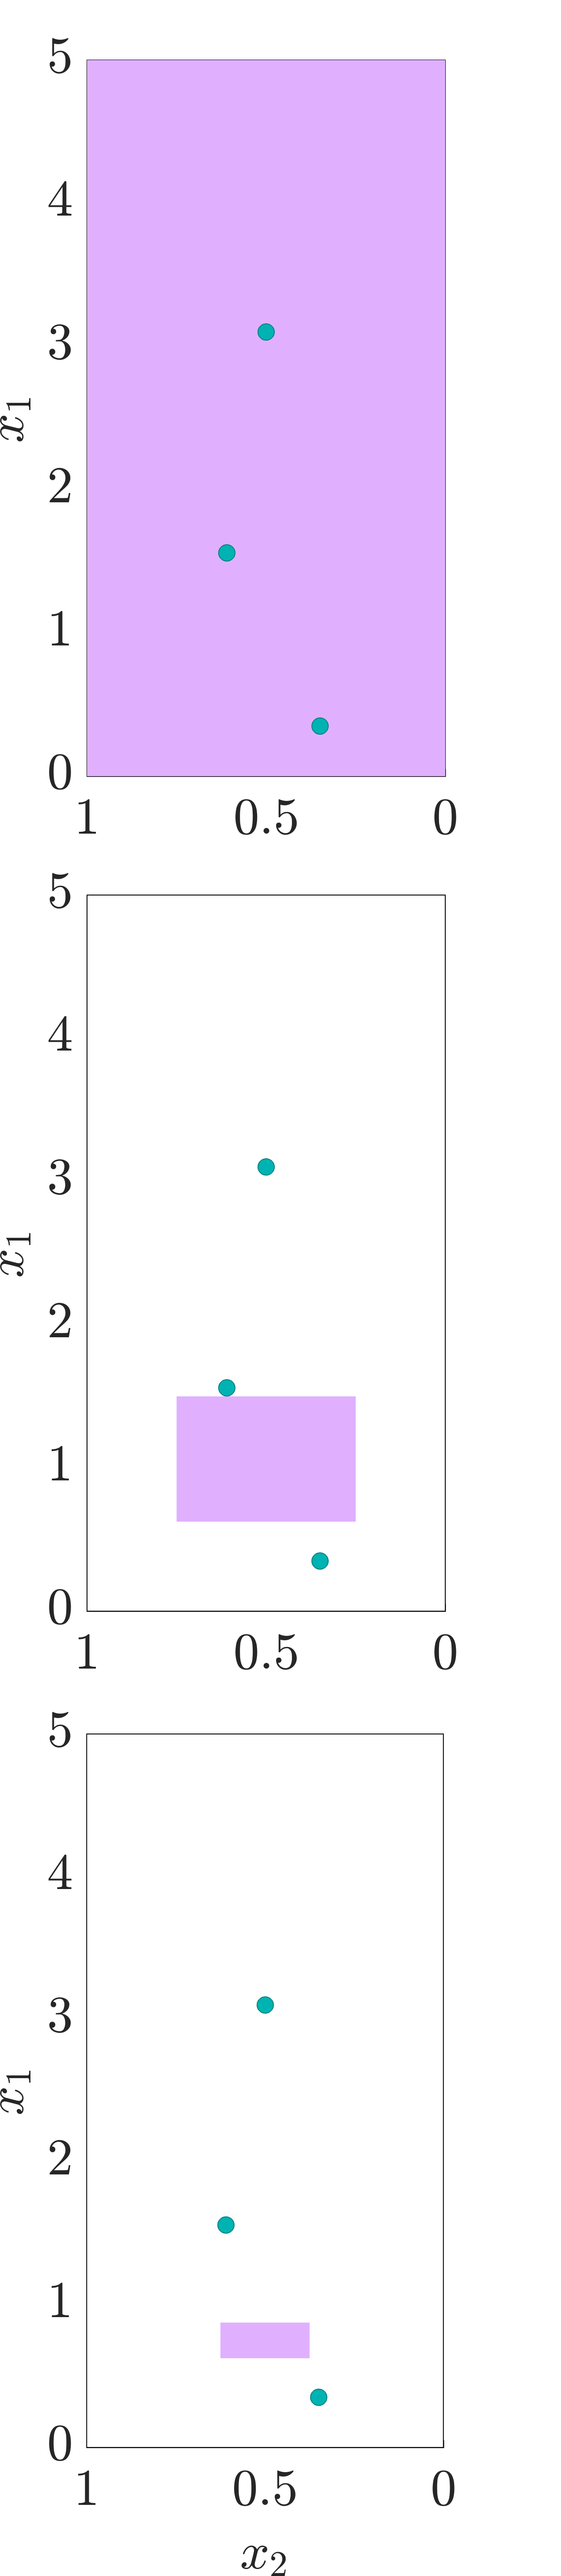
\includegraphics[width=0.23\textwidth]{vs_qoi/vs_qoi_setup.png}
  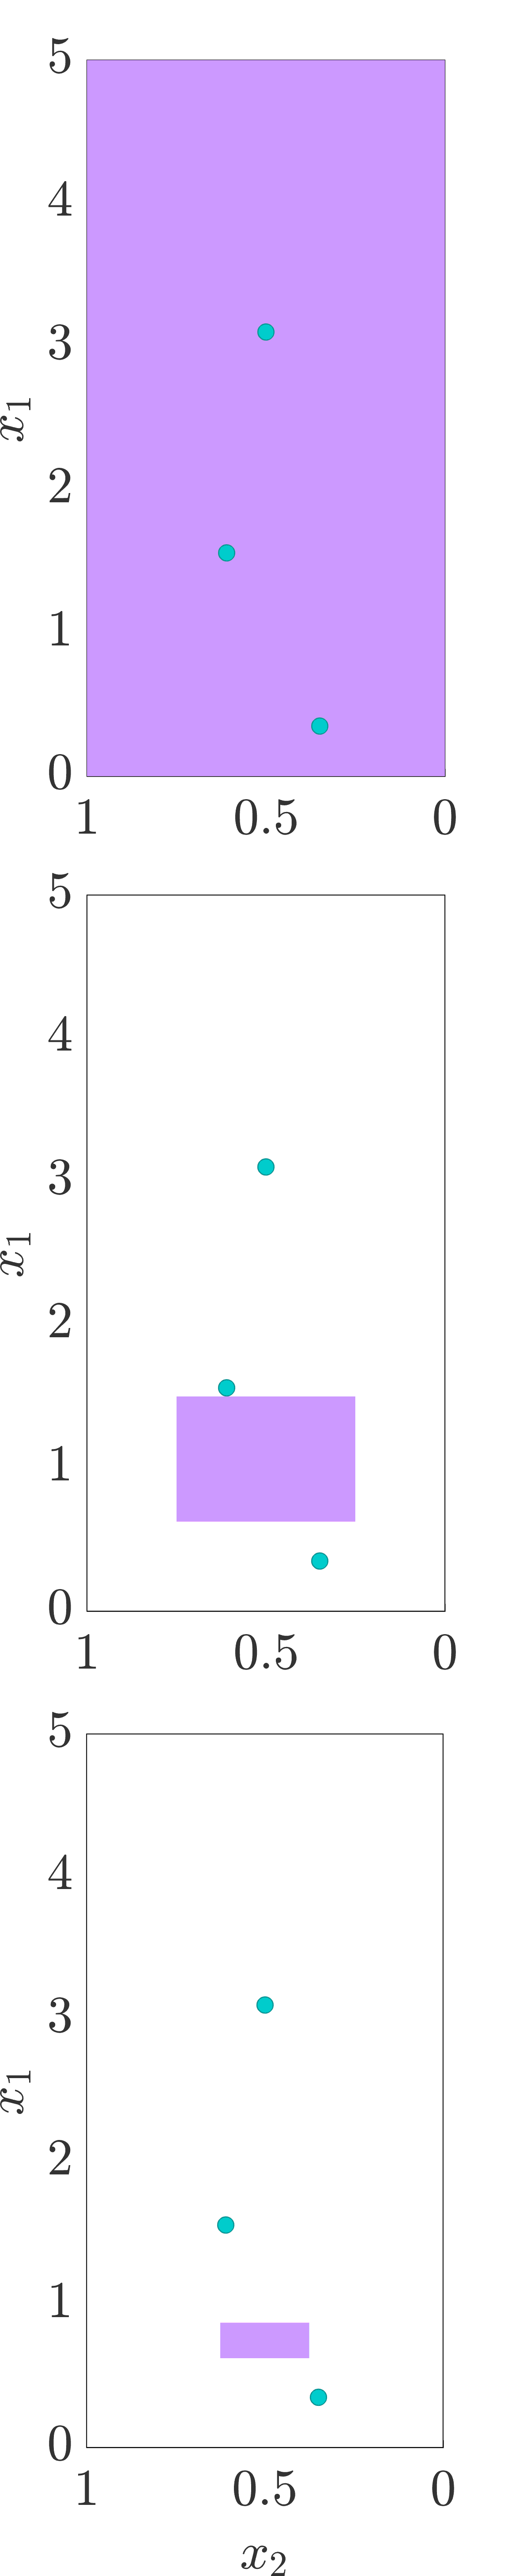
\includegraphics[width=0.21\textwidth]{vs_qoi/vs_qoi_setup_sidetrim.png}
  \label{subfig:obsSetup}
}
\captionsetup{justification=centering}
\subfloat[MF$_0$ ($0\%$ HF)][MF$_0$ \\($0\%$ HF)]{
  %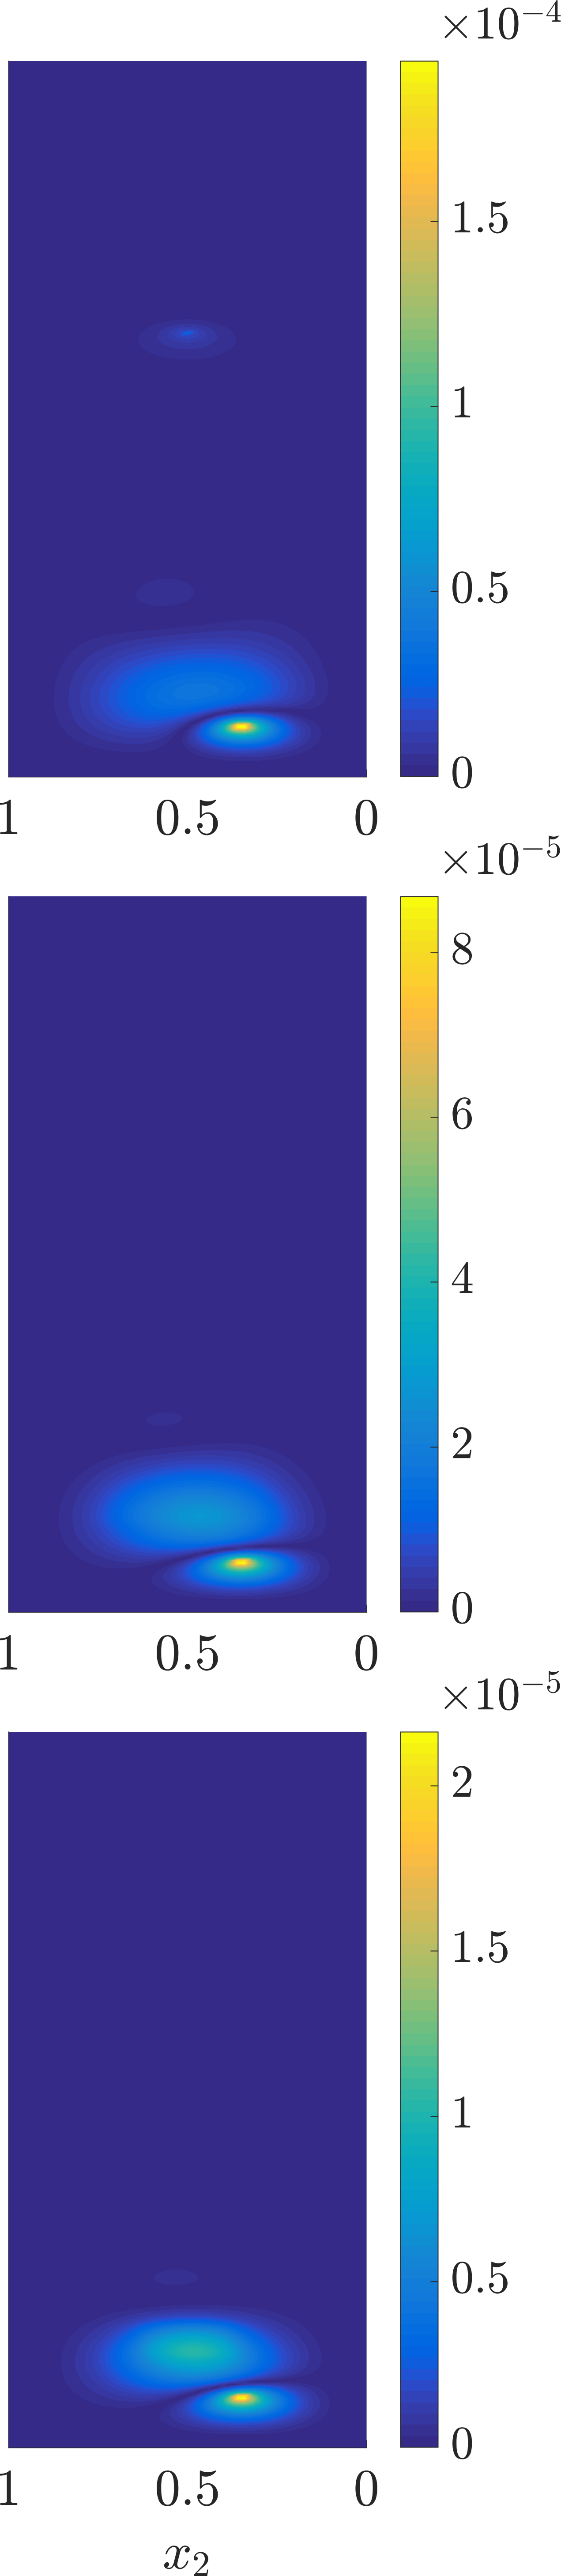
\includegraphics[width=0.23\textwidth]{vs_qoi/vs_qoi_err0.png}
  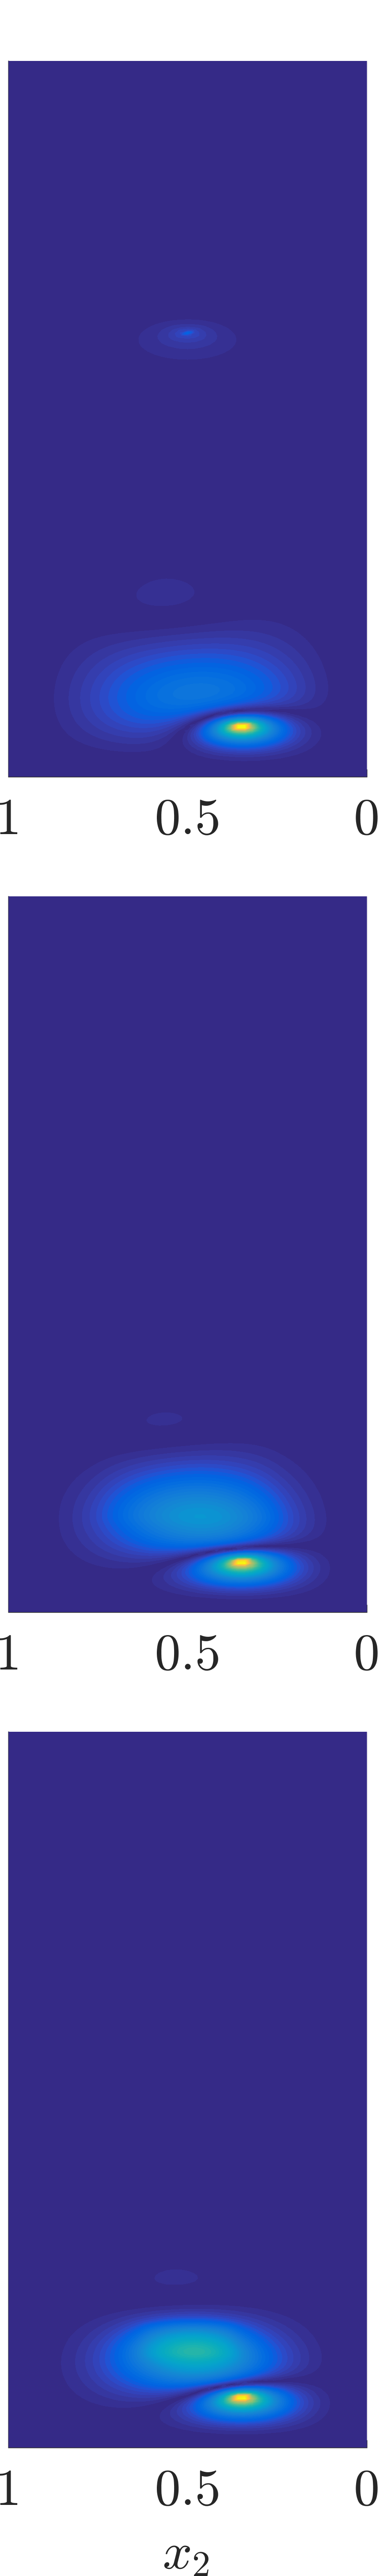
\includegraphics[width=0.16\textwidth]{vs_qoi/vs_qoi_err0_nobar.png}
  \label{subfig:obsLF}
}
\captionsetup{justification=centering}
\subfloat[MF$_1$ ($\sim5\%$ HF)][MF$_1$ \\($\sim5\%$ HF)]{
  %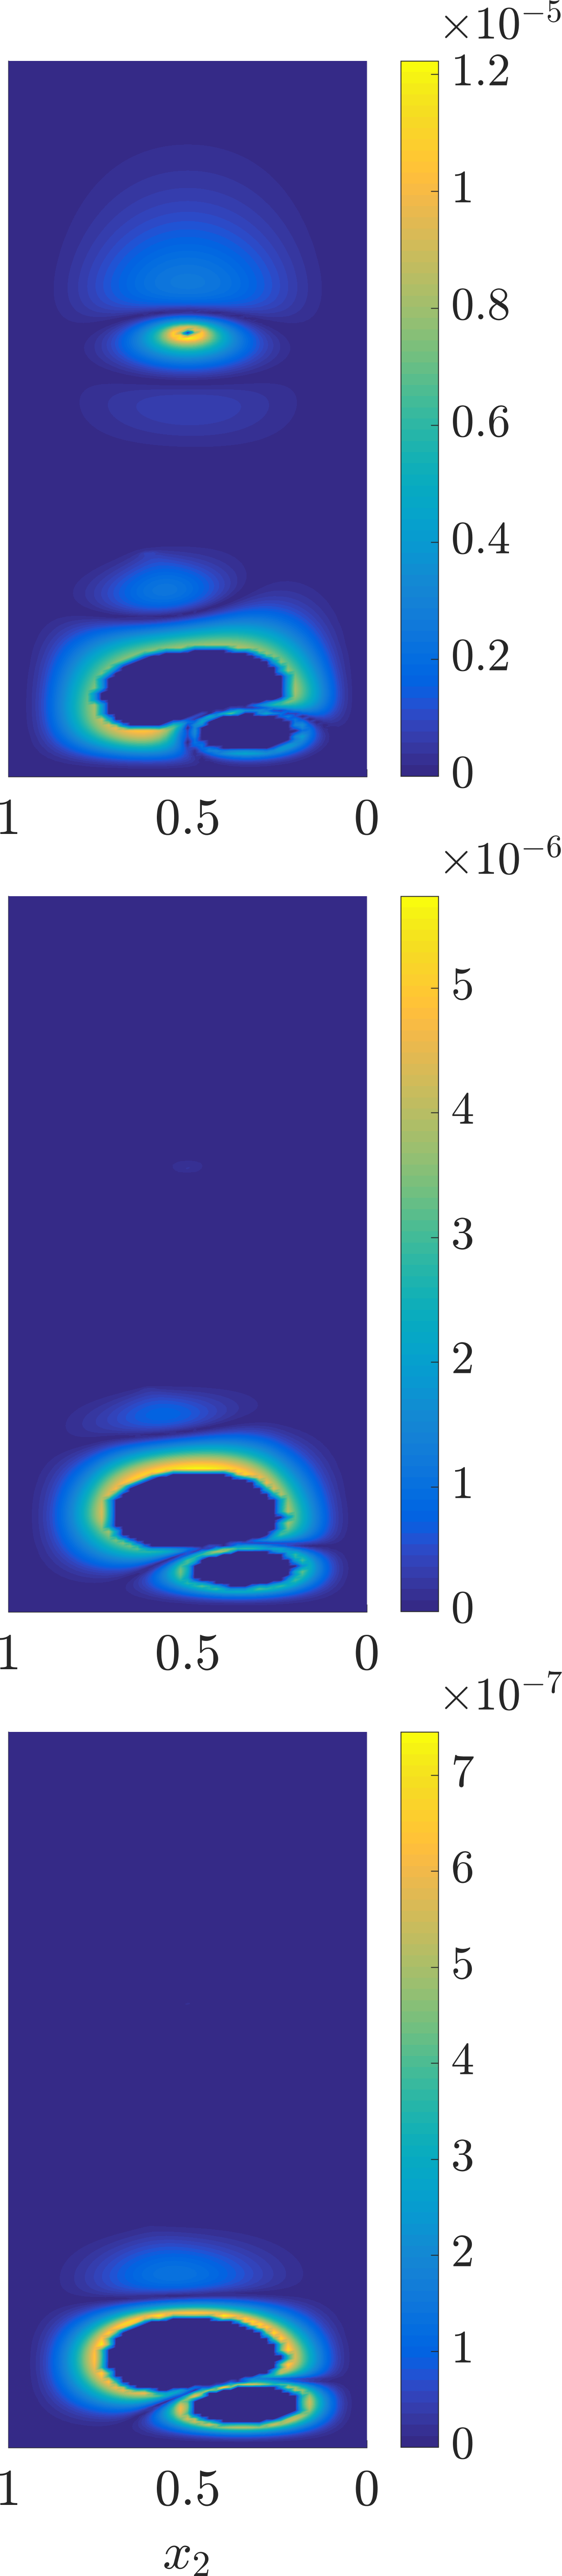
\includegraphics[width=0.23\textwidth]{vs_qoi/vs_qoi_err1.png}
  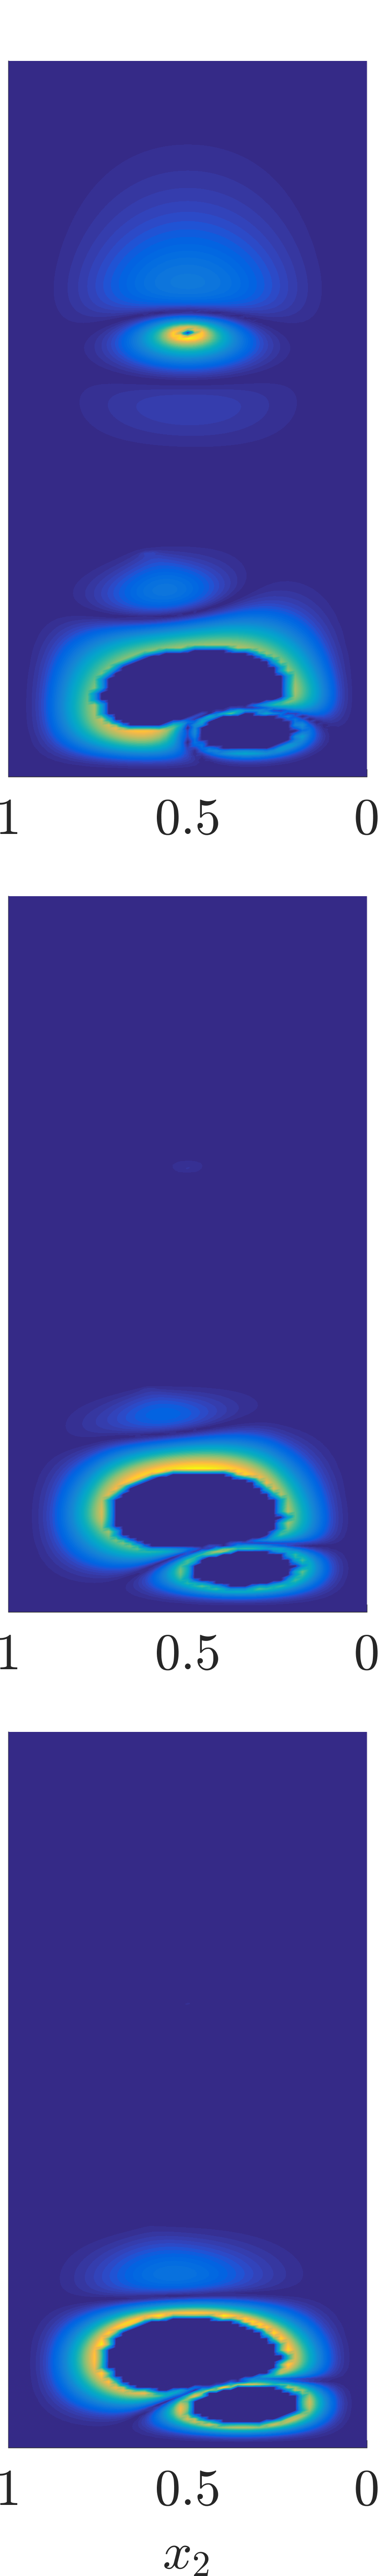
\includegraphics[width=0.16\textwidth]{vs_qoi/vs_qoi_err1_nobar.png}
}
\captionsetup{justification=centering}
\subfloat[MF$_2$ ($\sim10\%$ HF)][MF$_2$ \\($\sim10\%$ HF)]{
  %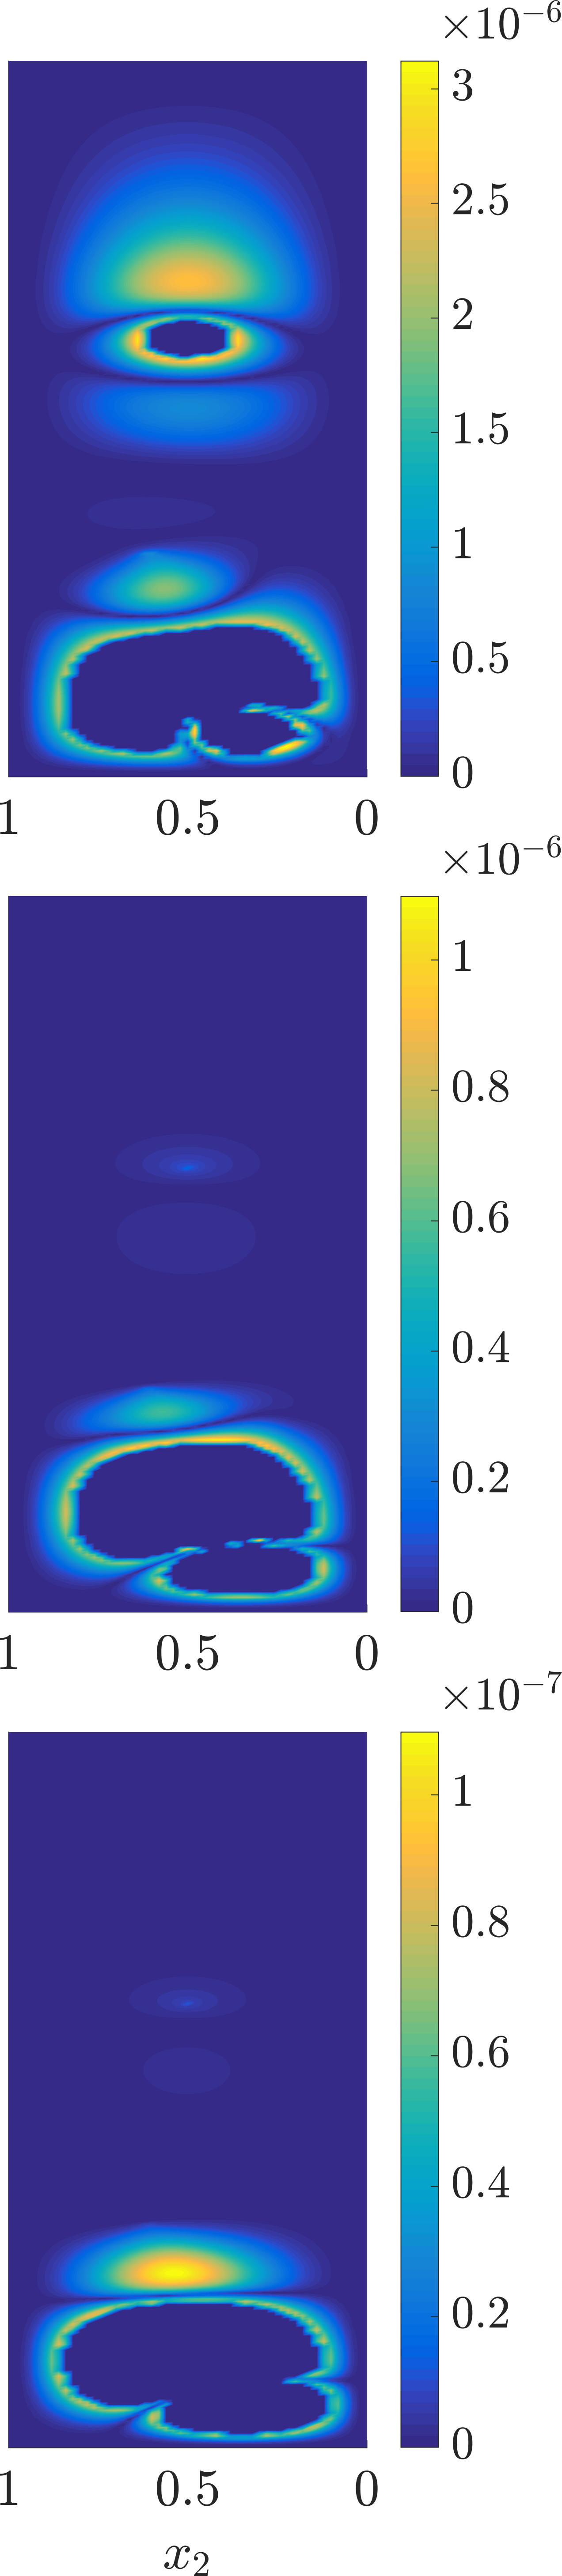
\includegraphics[width=0.23\textwidth]{vs_qoi/vs_qoi_err2.png}
  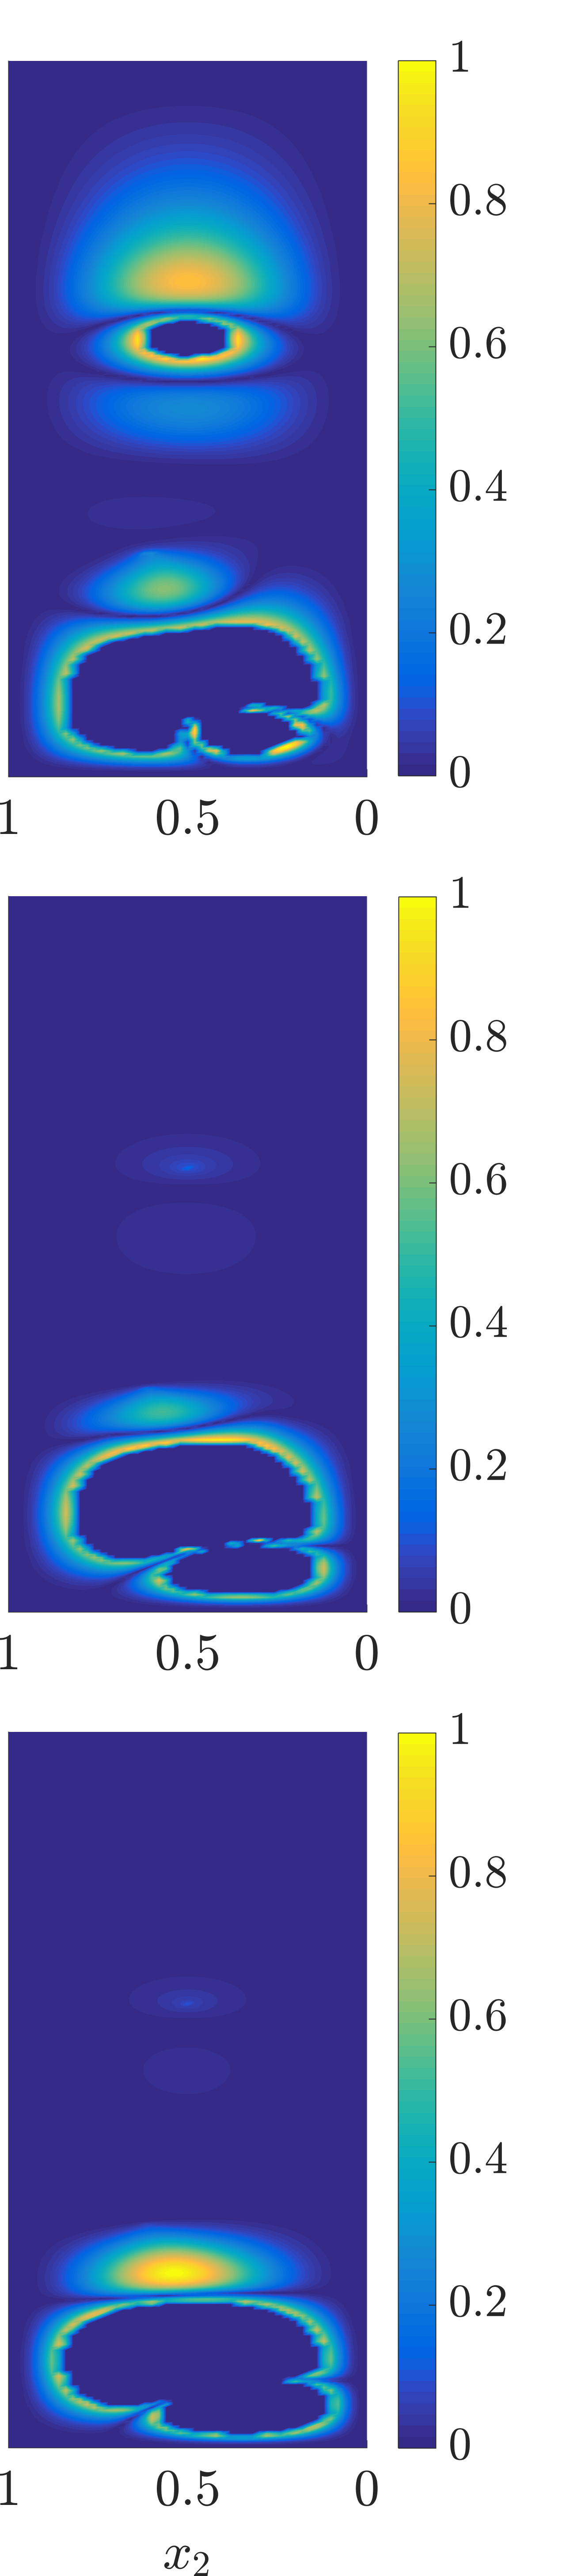
\includegraphics[width=0.23\textwidth]{vs_qoi/vs_qoi_err2_barnorm.png}
  \label{subfig:obsMFlast}
}
  \caption{Effects of increasing the QoI region. Column \protect\subref{subfig:obsSetup}: configuration of observations (teal points) and QoI region (purple box). Columns \protect\subref{subfig:obsLF}--\protect\subref{subfig:obsMFlast}): the relative error estimate decompositions for different mixed-fidelity models, relative to the largest localized error contribution; note the locations of regions of relatively large error compared to the observation locations and QoI region.}
  \label{fig:qoiStudy}
\end{figure}

\Cref{fig:dataStudy} shows another set of cases considered, now with the same QoI region $\Omega_I$ but with increasing, nested sets of observations.
The error decomposition for the three cases is shown in \Cref{fig:dataStudy}. The bottom row is the same as that in \Cref{fig:qoiStudy}. Refinement appears to be consistently most important around the observation location closest to $x_1=0$ and the QoI region. However, as more observation locations are added, it becomes no longer necessarily true that refinement becomes less important around observation locations as their distance from the QoI region increases. In the second and third rows, one can see that after the areas around the QoI region and the two closest observation locations have been refined, the next area to be refined is not around the third closest observation location, but rather around one near the middle of the domain. This suggests that interactions between observation locations and the QoI may be non-intuitive, and in these cases a rigorous method for forming a mixed-fidelity model would be most helpful. % KW: I don't understand a lot of this discussion. You need to explain to me what you mean.

\begin{figure}[htbp]
\centering
\captionsetup{justification=centering}
\subfloat[Locations of observations and QoI region $\Omega_I$][Locations of \\observations and \\QoI region $\Omega_I$]{
  %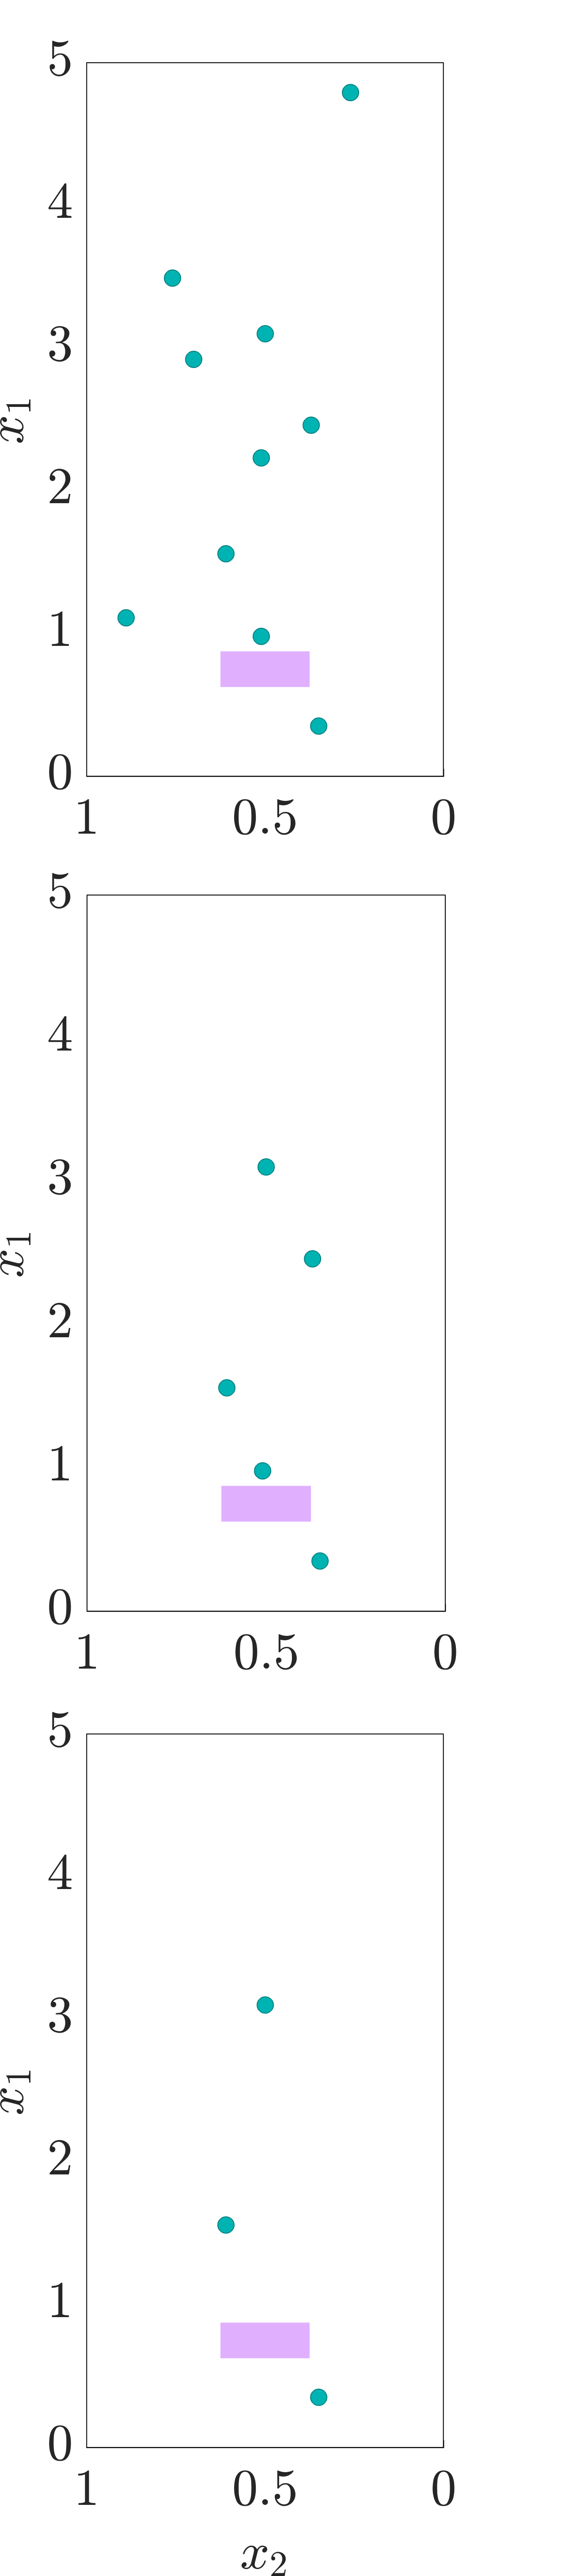
\includegraphics[width=0.23\textwidth]{vs_data/vs_data_setup.png}
  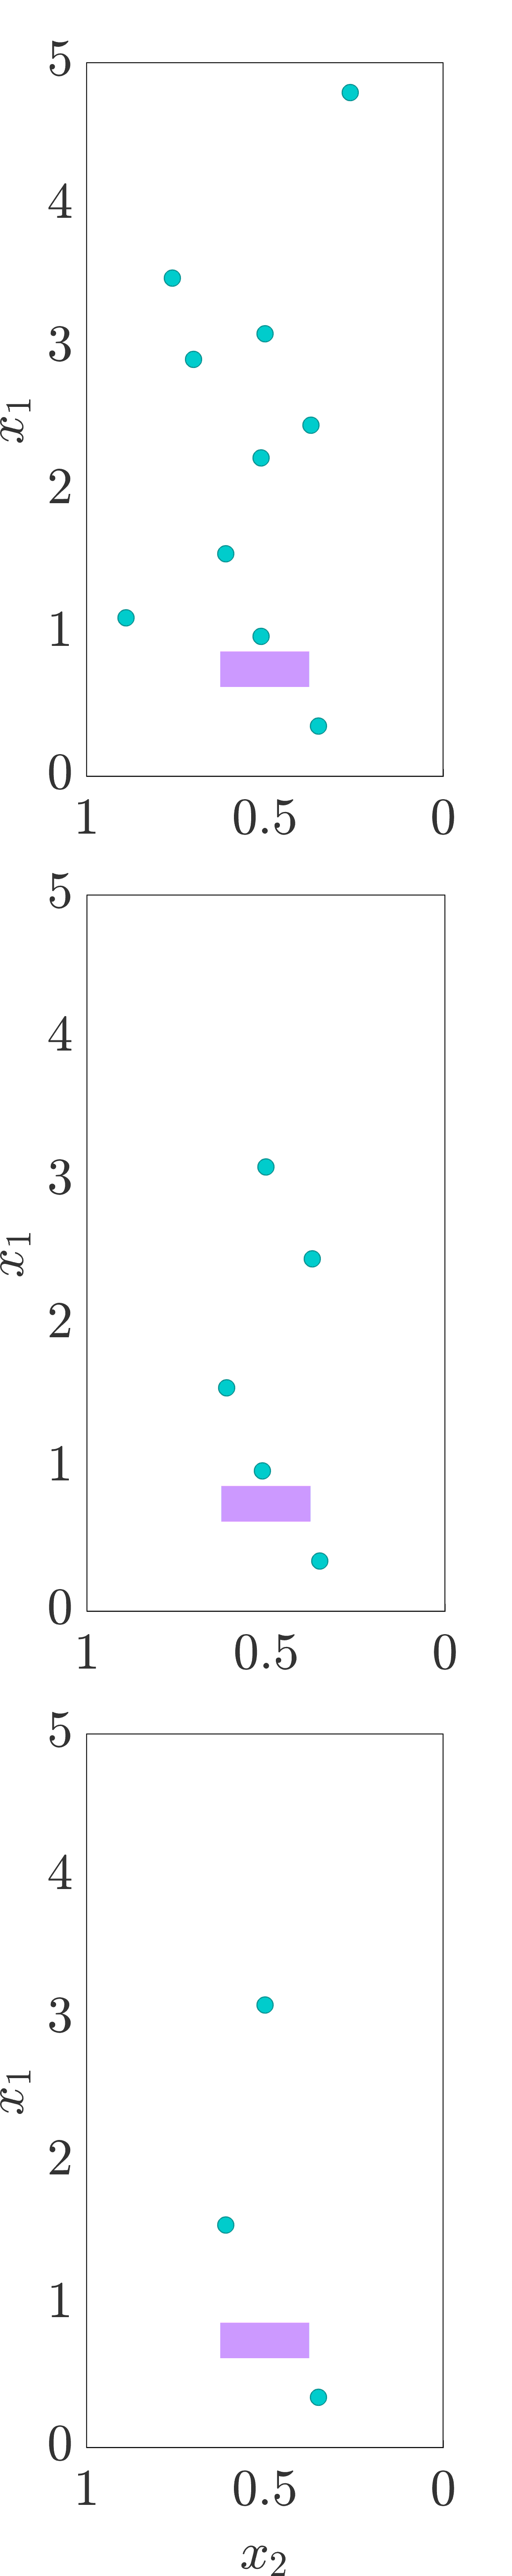
\includegraphics[width=0.21\textwidth]{vs_data/vs_data_setup_sidetrim.png}
  \label{subfig:obsSetup2}
}
\captionsetup{justification=centering}
\subfloat[MF$_0$ ($0\%$ HF)][MF$_0$ \\($0\%$ HF)]{
  %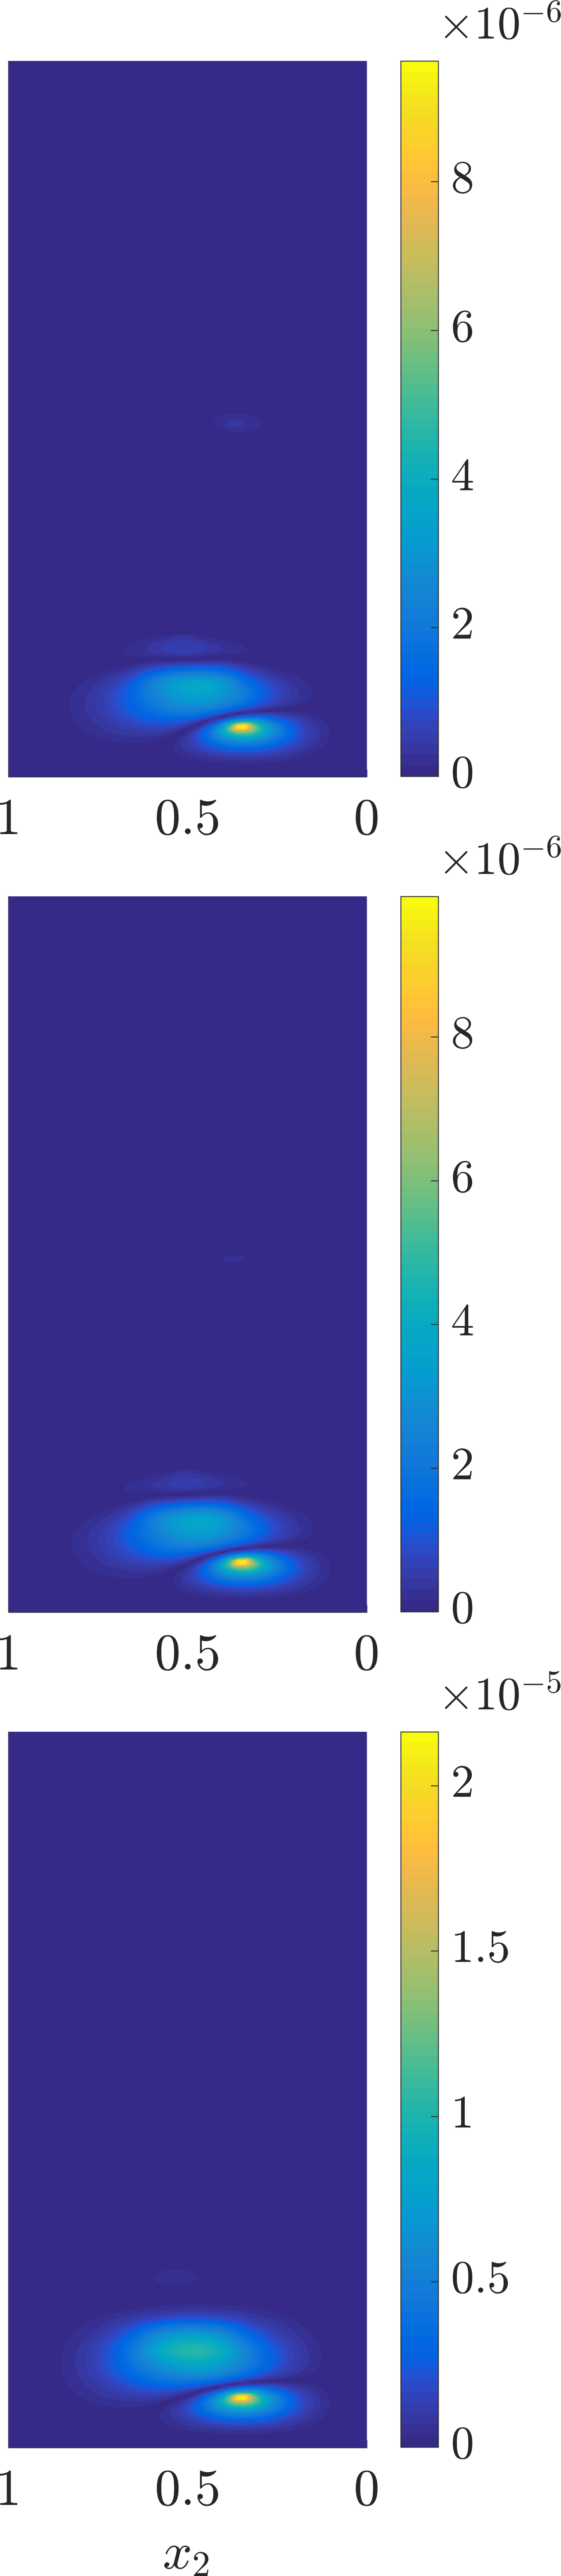
\includegraphics[width=0.23\textwidth]{vs_data/vs_data_err0.png}
  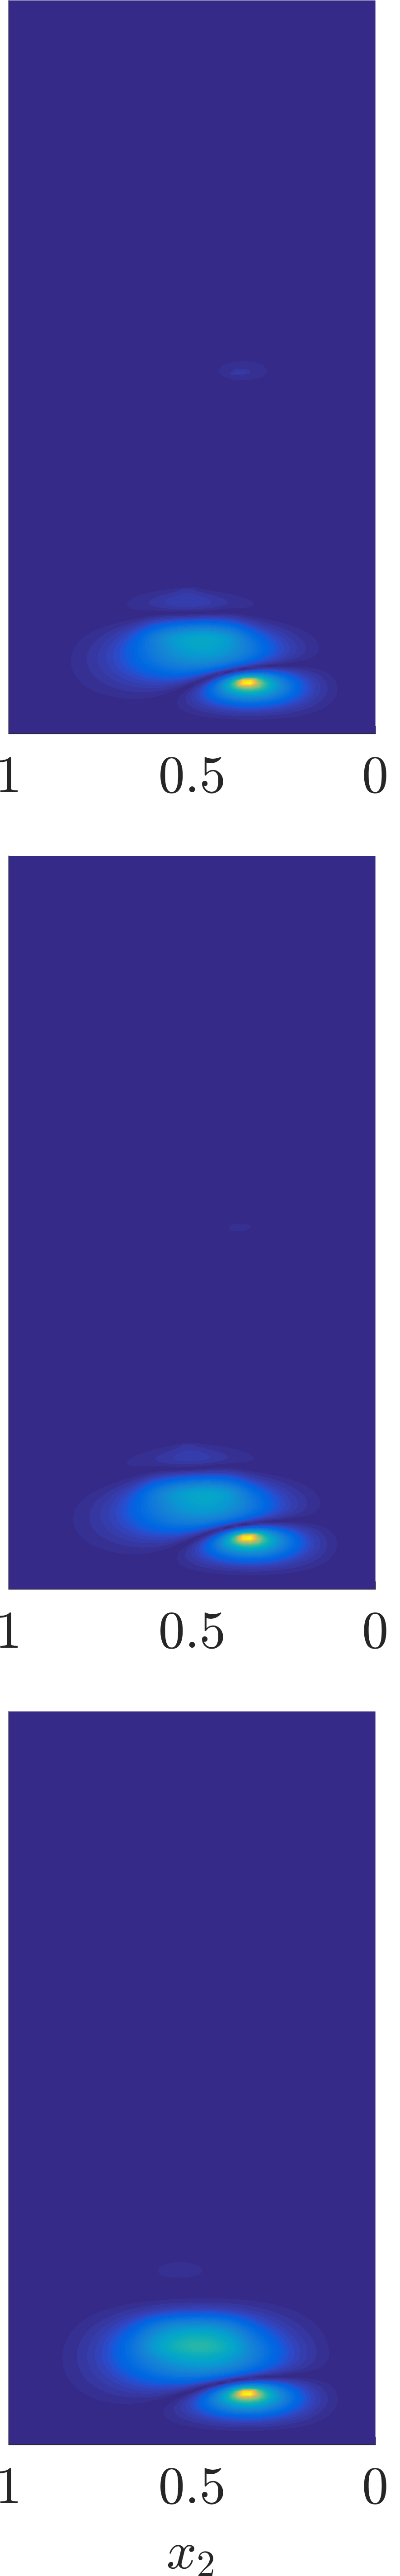
\includegraphics[width=0.16\textwidth]{vs_data/vs_data_err0_nobar.png}
  \label{subfig:obsLF2}
}
\captionsetup{justification=centering}
\subfloat[MF$_1$ ($\sim5\%$ HF)][MF$_1$ \\($\sim5\%$ HF)]{
  %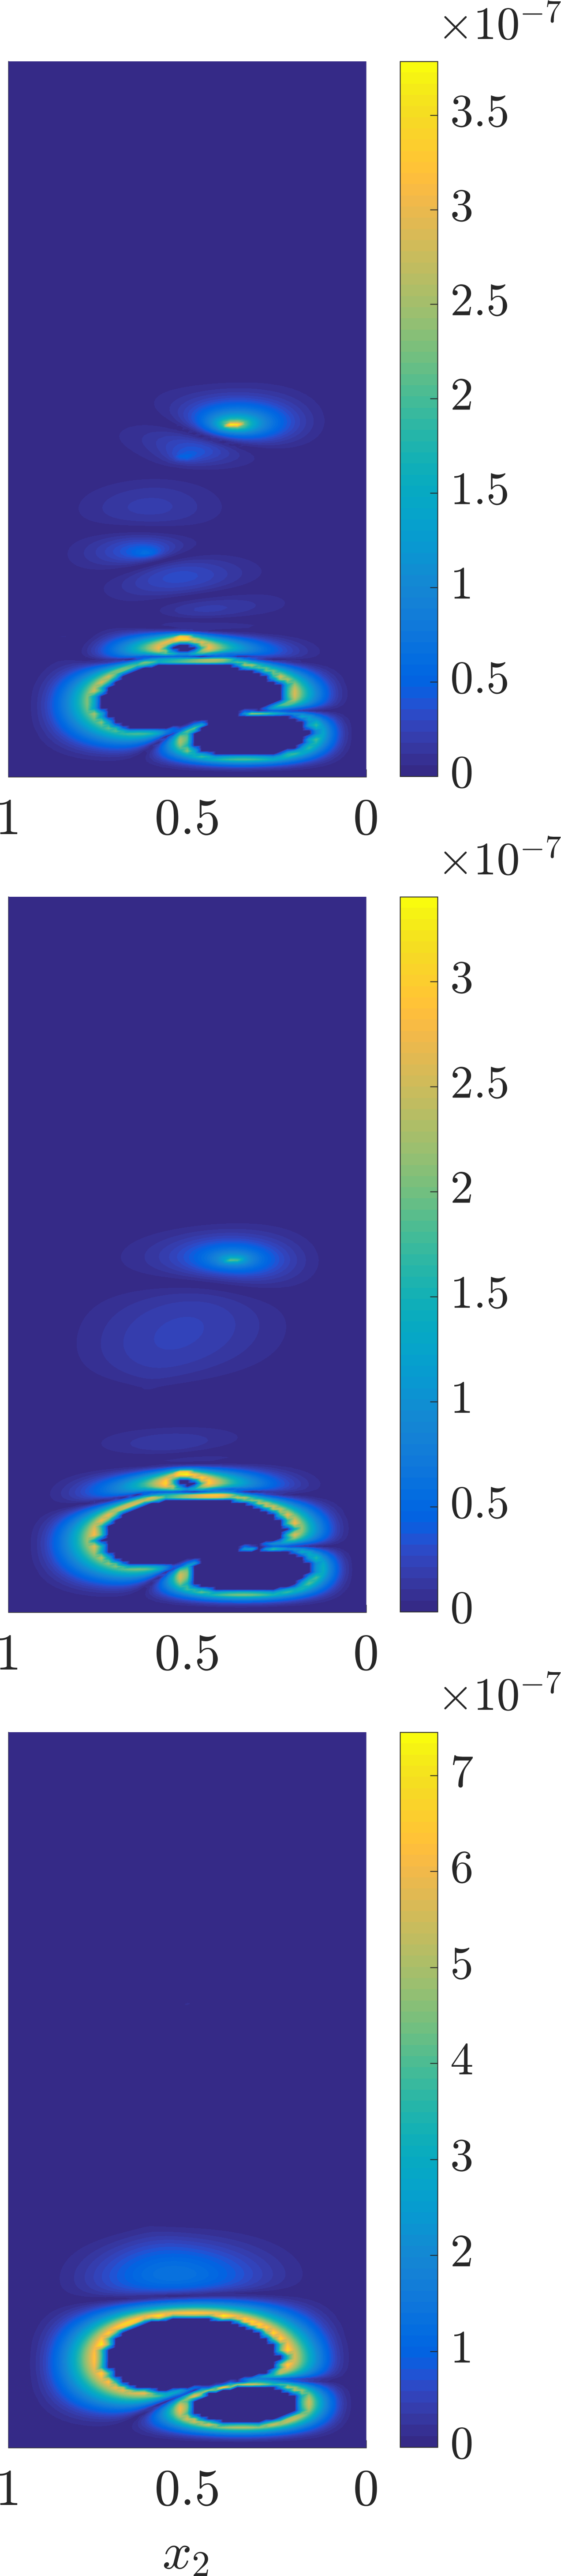
\includegraphics[width=0.23\textwidth]{vs_data/vs_data_err1.png}
  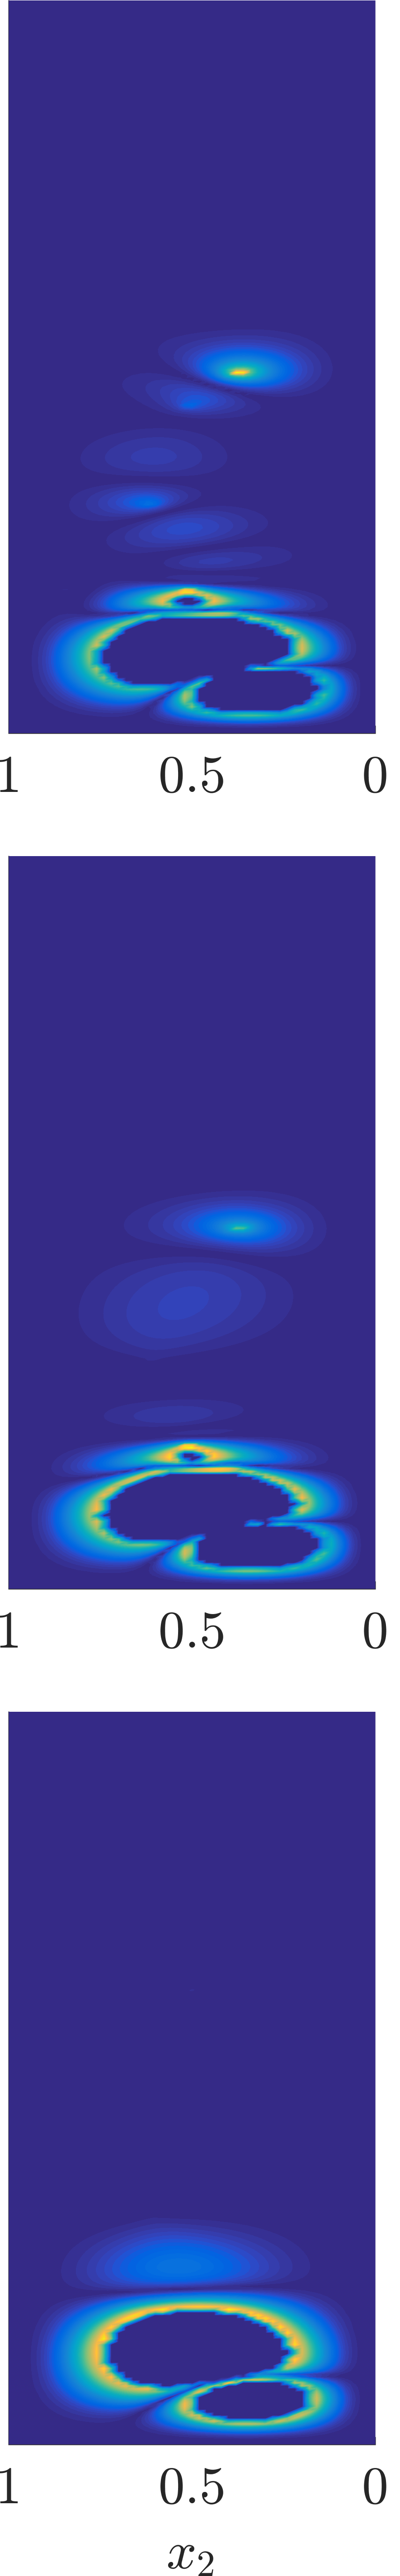
\includegraphics[width=0.16\textwidth]{vs_data/vs_data_err1_nobar.png}
}
\captionsetup{justification=centering}
\subfloat[MF$_2$ ($\sim10\%$ HF)][MF$_2$ \\($\sim10\%$ HF)]{
  %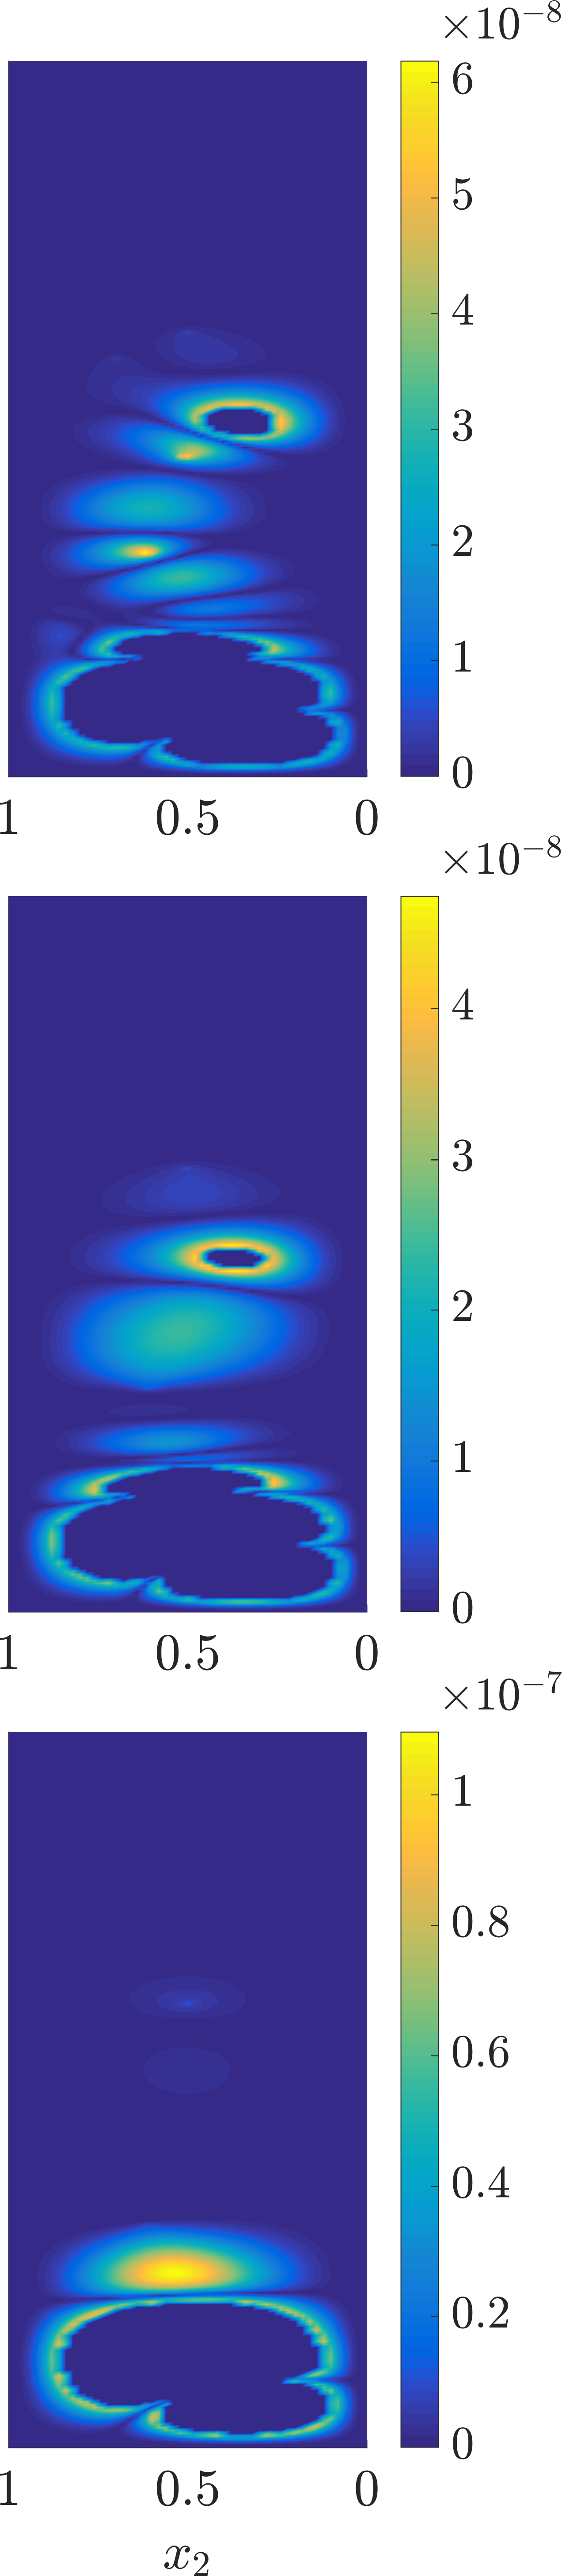
\includegraphics[width=0.23\textwidth]{vs_data/vs_data_err2.png}
  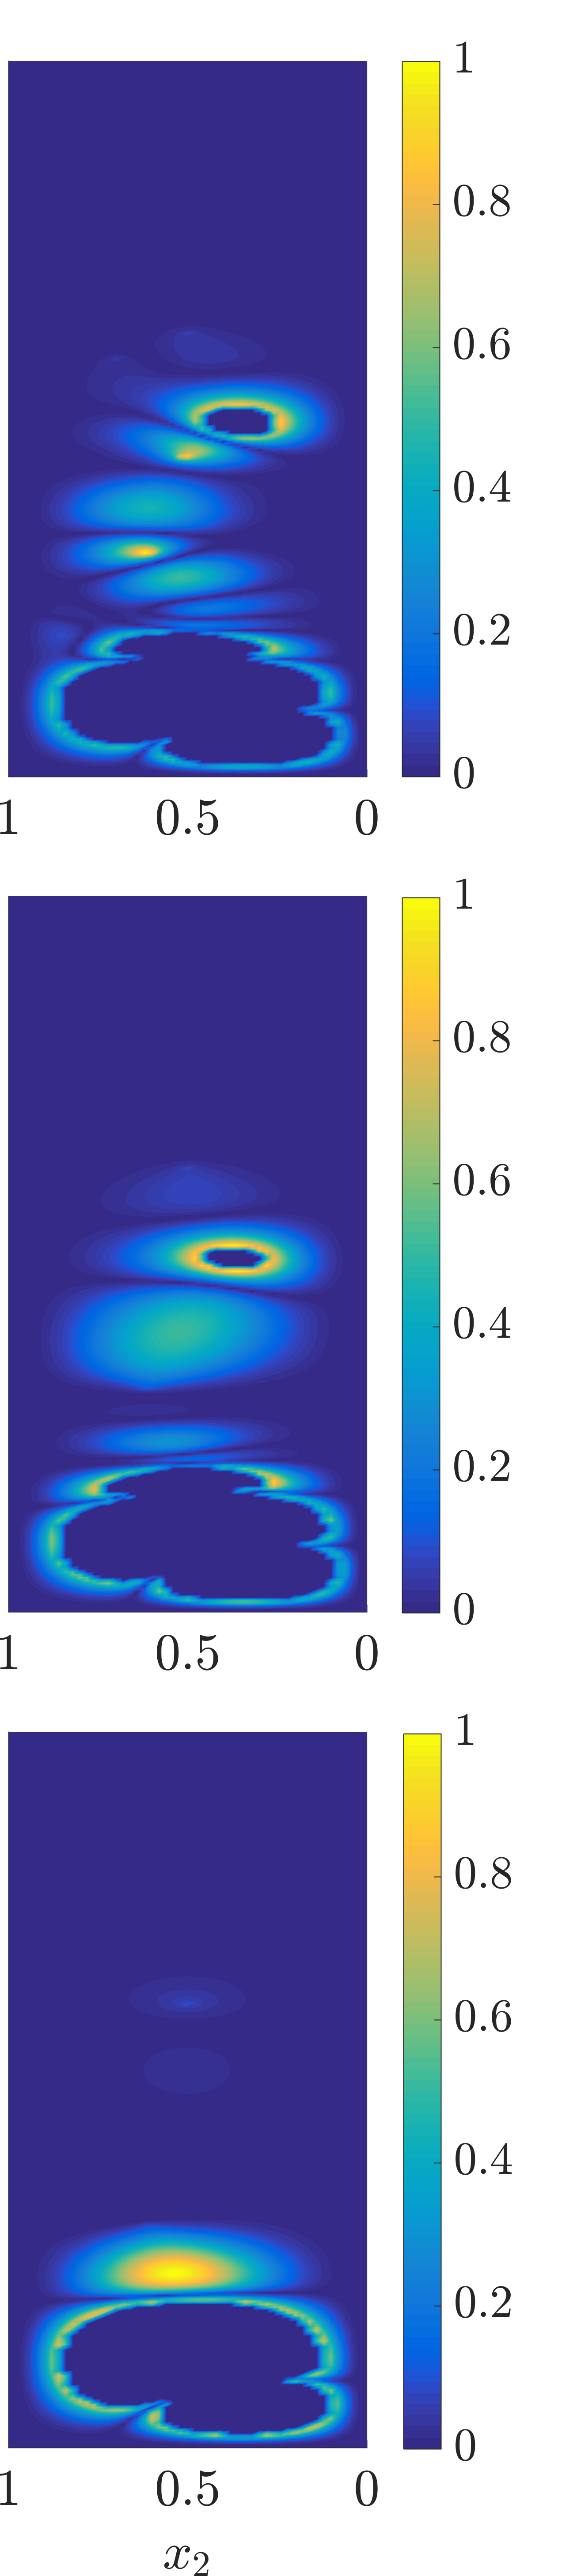
\includegraphics[width=0.23\textwidth]{vs_data/vs_data_err2_barnorm.png}
  \label{subfig:obsMFlast2}
}
  \caption{Effects of increasing the number of observations. Column \protect\subref{subfig:obsSetup2}: configuration of observations (teal points) and QoI region (purple box). Columns \protect\subref{subfig:obsLF2}--\protect\subref{subfig:obsMFlast2}): the relative error estimate decompositions for different mixed-fidelity models, relative to the largest localized error contribution; note the locations of regions of relatively large error compared to the observation locations and QoI region.}
  \label{fig:dataStudy}
\end{figure}

%------------------------------------------------------------------------------------------------------------------------%
\subsection{Variable Parameterization: Constant vs.\ Field Parameters} \label{sec:constvfield}
%------------------------------------------------------------------------------------------------------------------------%

In this subsection, we consider two models which differ in the space to which the parameter belongs, with the low-fidelity model having fewer degrees of freedom. 

%------------------------------------------------------------%
\subsubsection{Problem Setup}
%------------------------------------------------------------%

We consider the same high-fidelity model as in \Cref{sec:cdvcdr}:
\begin{equation}
k_d\nabla^2 u - \vec{V}\cdot\nabla u + k_ru^2= f(q),\quad q\in U,
\end{equation}
with the same diffusion coefficient $k_d = 0.1$  and reaction coefficient $k_r = -42$. The low-fidelity model
\begin{equation}
k_d\nabla^2 u - \vec{V}\cdot\nabla u + k_ru^2= f(q),\quad q\in\R
\end{equation}
differs from the high-fidelity model only in that the parameter $q$ is a constant instead of a field. The intermediate mixed-fidelity models thus have parameter fields that are constant over the subregions of the domain where the low-fidelity model is used. For ease of implementation, we require that the resulting parameter field remain continuous at the interface between the low-fidelity and high-fidelity subdomains, although this constraint is not necessary for the theory to hold. The domain, mesh, boundary conditions, and velocity field, as well as the observations, unknown parameters to be inferred, and QoI, remain the same as described in \Cref{sec:cdvcdr}. As the inverse problem is ill-posed, except when the low-fidelity model is used throughout the domain, regularization is used; the Tikhonov regularization term in \Cref{eq:invOpt_obj} is $R(q)=\frac{\beta}{2}\int_\Omega \|\nabla f(q)\|_2^2+f(q)^2\:\textrm{d}A$, where $\beta=10^{-3}$ is a regularization coefficient. 

%------------------------------------------------------------%
\subsubsection{Adaptive Model Refinement Results}
%------------------------------------------------------------%

As with the previous examples in \Cref{sec:cdvcdr}, the decomposition of the error estimate is used to select additional regions of the domain in which to use the high-fidelity model. The number of degrees of freedom in the inverse problem increases with the proportion of the domain in which the high-fidelity model is used. With each iteration, an additional $10\%$ of the elements are marked for refinement. This is repeated until the estimated absolute relative error in the QoI is less than $1\%$.

\Cref{fig:svfRef} shows the local error contributions, as well as the subdomains where the low- and high-fidelity models are used, for the first two and last mixed-fidelity model thus generated. 
%
\begin{figure}[htbp]
\centering
\subfloat[MF$_0$ ($0\%$ HF)]{
	\includegraphics[width=0.46\textwidth]{svf/cd_cdr_LF_divvy.png}
  \includegraphics[width=0.49\textwidth]{svf/err_breakdown_LF.png}
} \\
\subfloat[MF$_1$ ($10\%$ HF)]{
	\includegraphics[width=0.46\textwidth]{svf/cd_cdr_MF01_divvy.png}
  \includegraphics[width=0.49\textwidth]{svf/err_breakdown_MF01.png}
} \\
\subfloat[MF$_2$ ($20\%$ HF)]{
  \includegraphics[width=0.46\textwidth]{svf/cd_cdr_MF02_divvy.png}
  \includegraphics[width=0.49\textwidth]{svf/err_breakdown_MF02.png}
} \\
%\begin{subfigure}[b]{\textwidth}
%	\centering
%	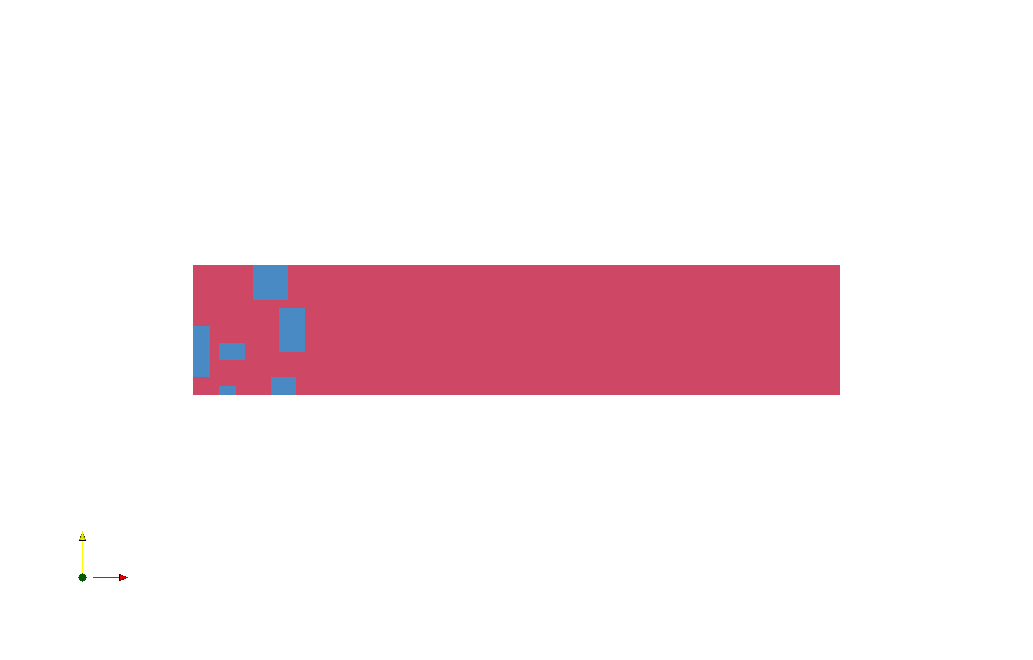
\includegraphics[width=0.48\textwidth]{svf/cd_cdr_MF03_divvy.png}
%  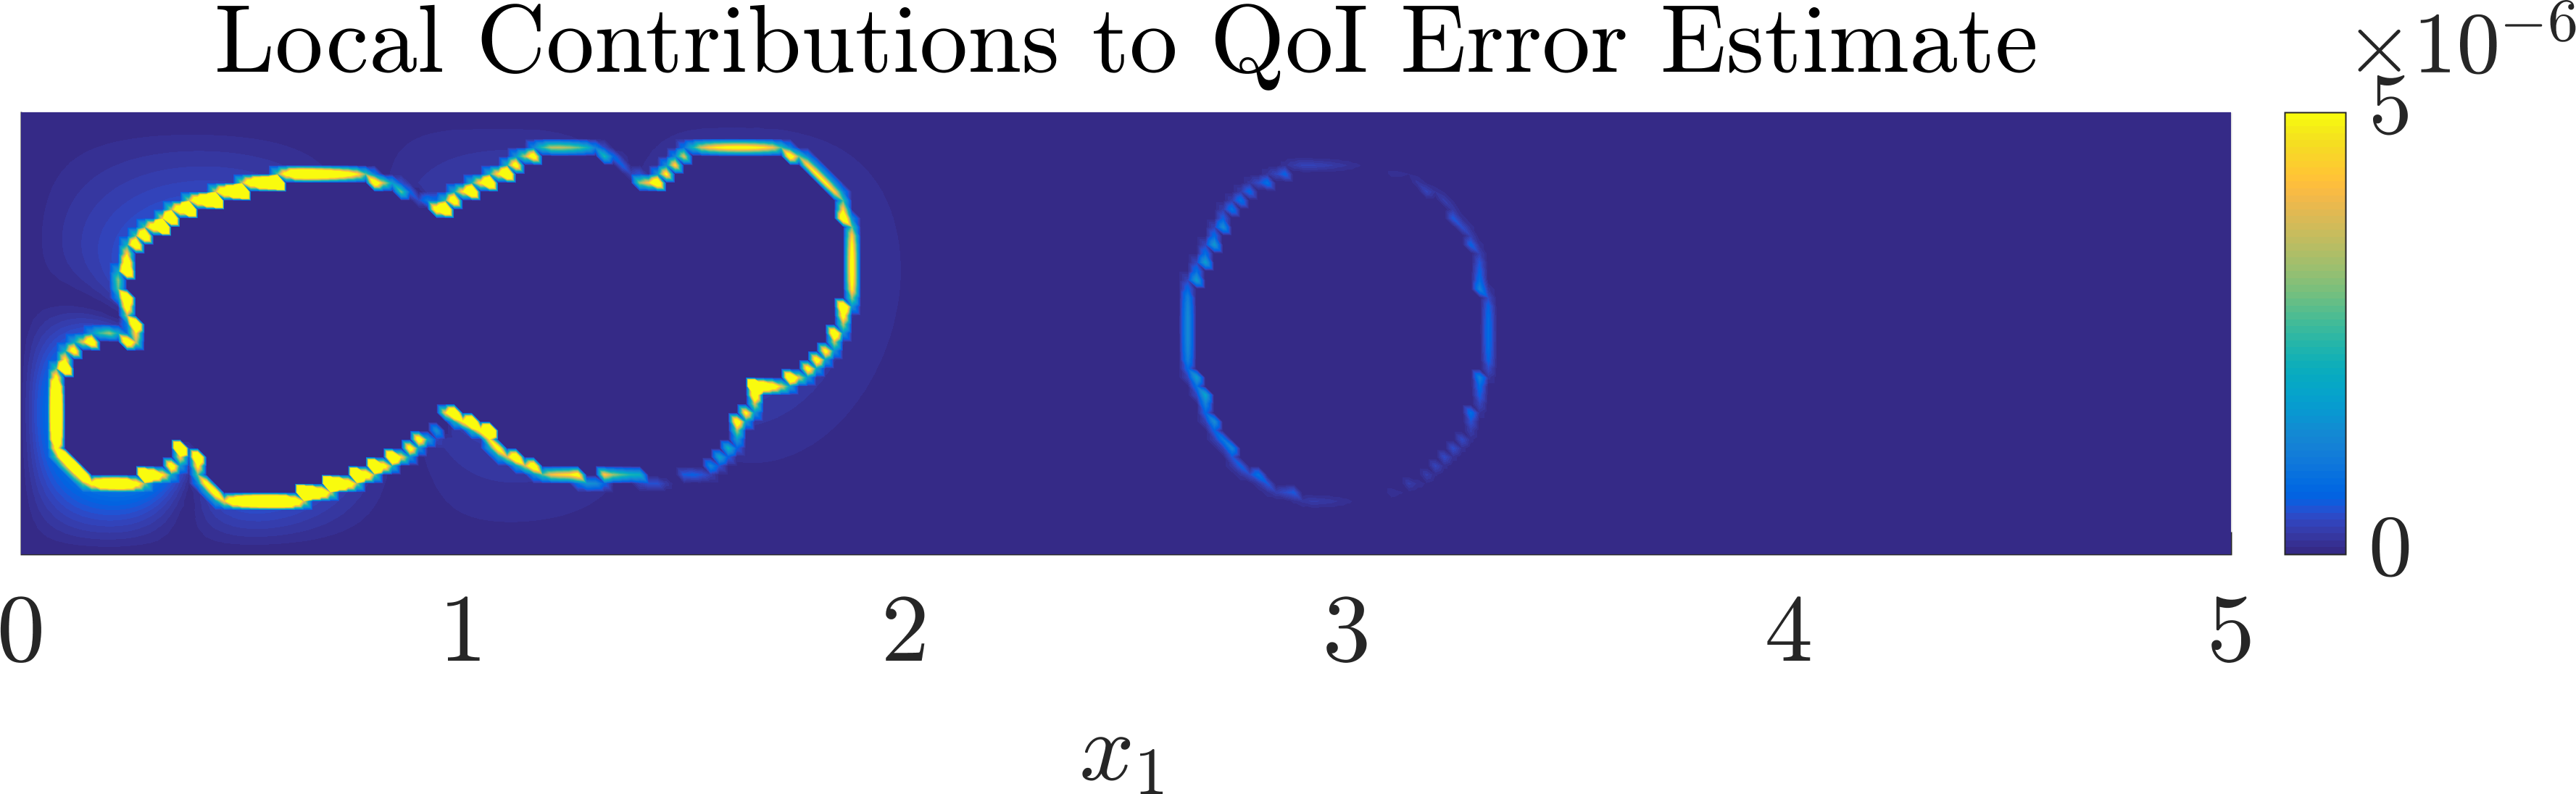
\includegraphics[width=0.51\textwidth]{svf/err_breakdown_MF03.png}
%  \vspace{-0.7\baselineskip}
%  \caption{MF$_3$ ($30\%$ HF)}
%  \vspace{0.8\baselineskip}
%\end{subfigure}
%\begin{subfigure}[b]{\textwidth}
%	\centering
%	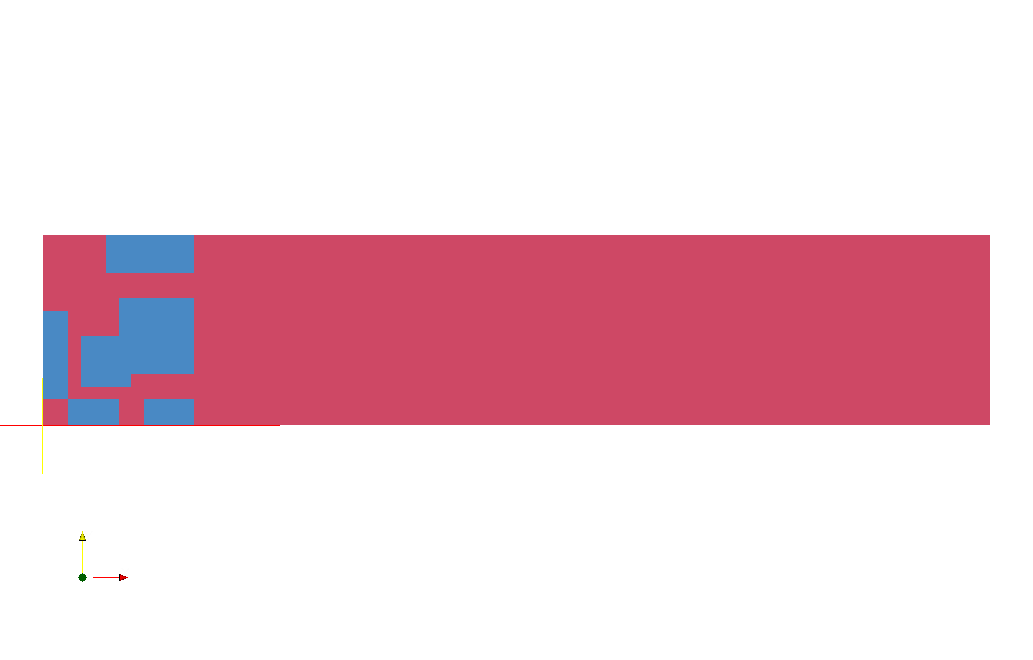
\includegraphics[width=0.48\textwidth]{svf/cd_cdr_MF04_divvy.png}
%  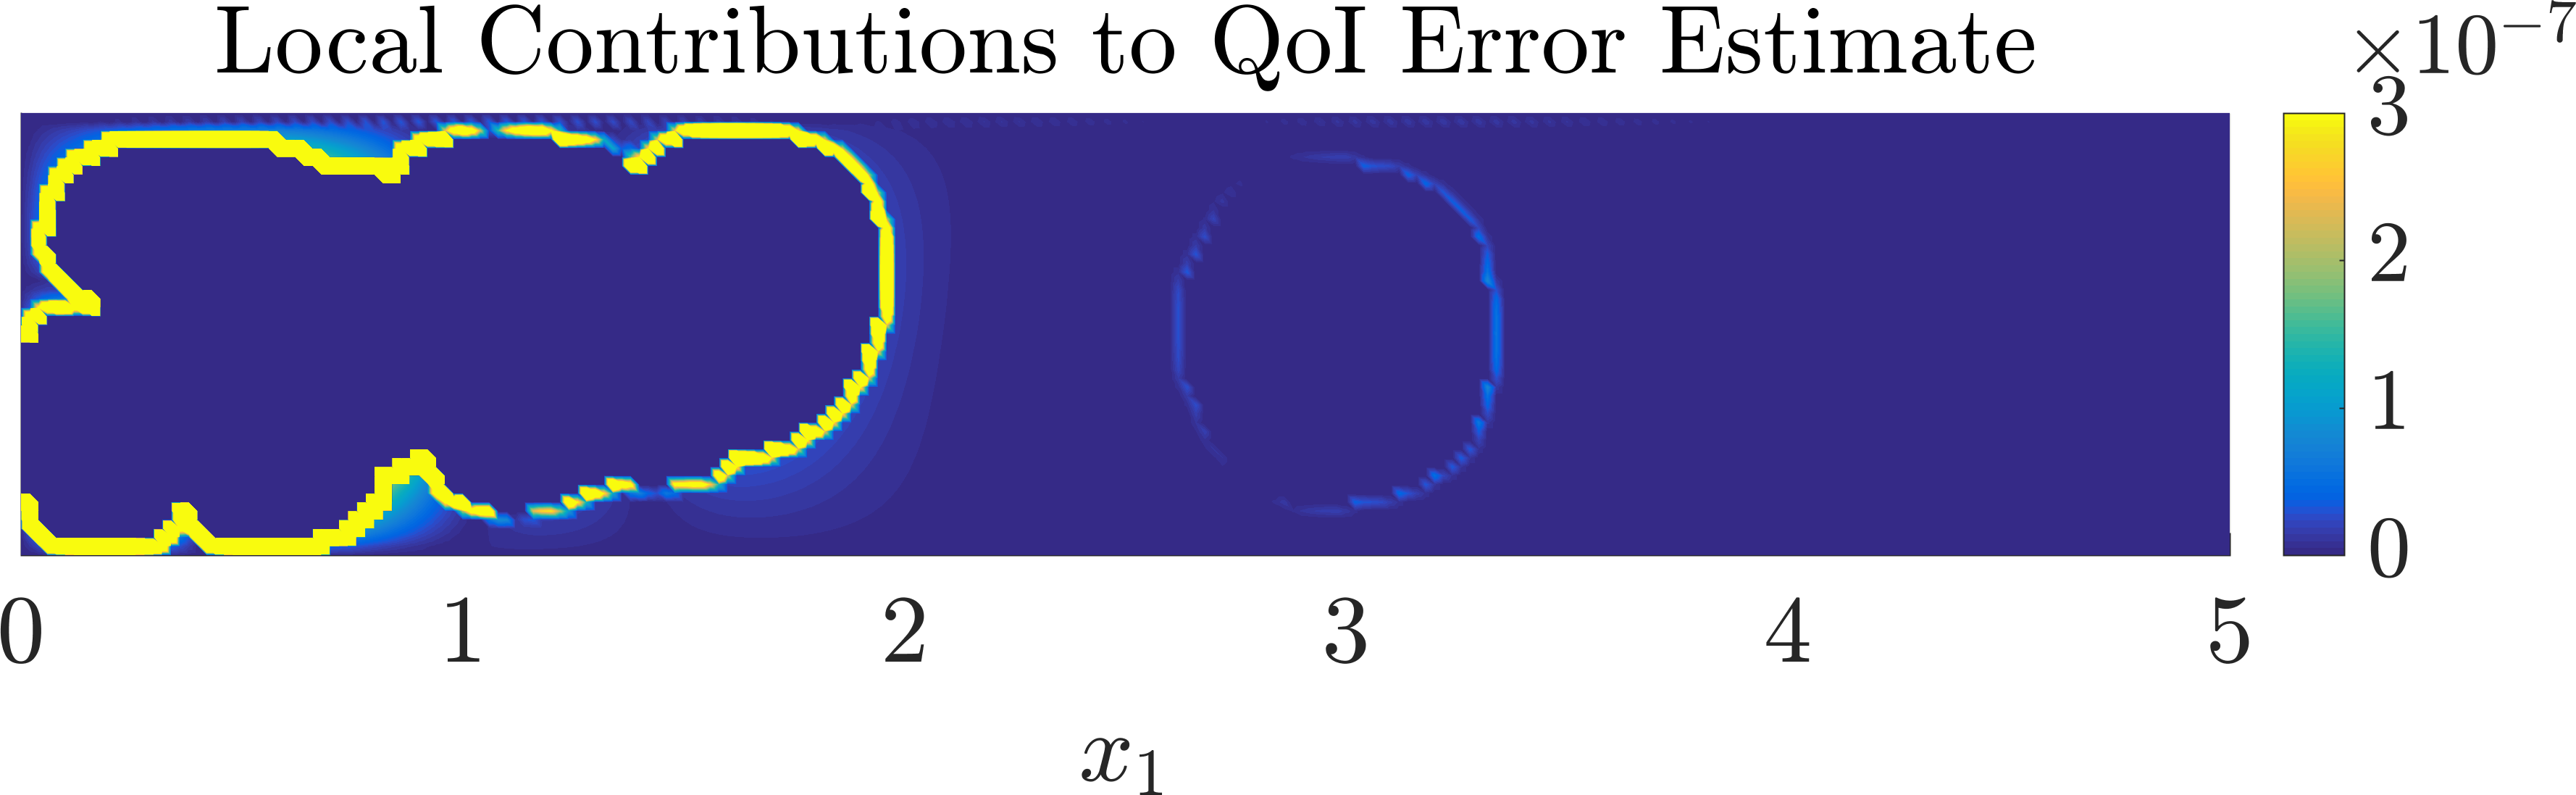
\includegraphics[width=0.51\textwidth]{svf/err_breakdown_MF04.png}
%  \vspace{-0.7\baselineskip}
%  \caption{MF$_4$ ($40\%$ HF)}
%  \vspace{0.8\baselineskip}
%\end{subfigure}
%\begin{subfigure}[b]{\textwidth}
%	\centering
%	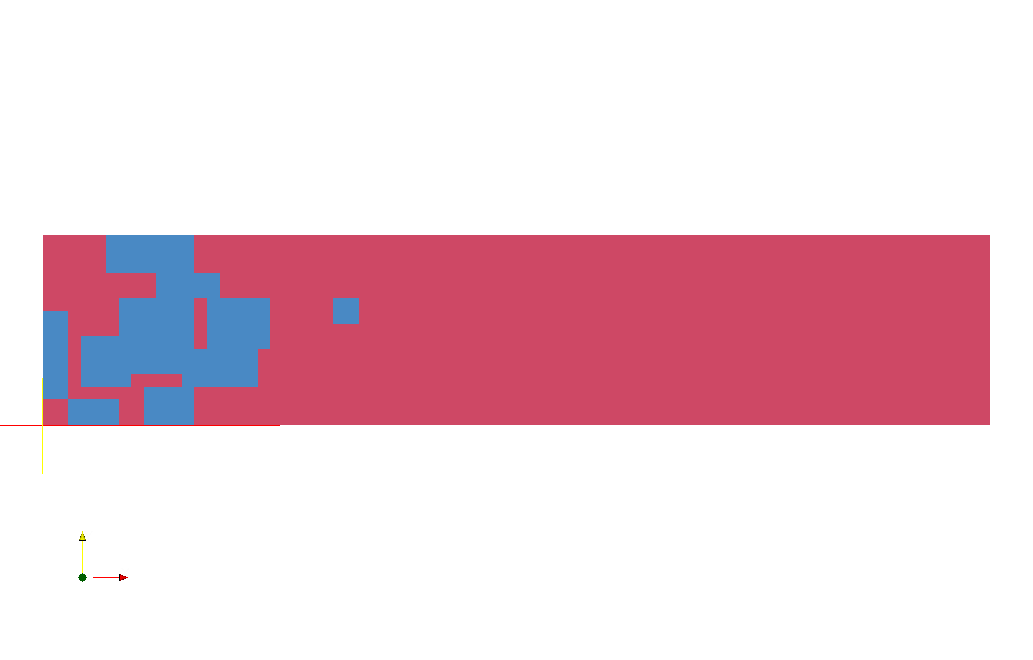
\includegraphics[width=0.48\textwidth]{svf/cd_cdr_MF05_divvy.png}
%  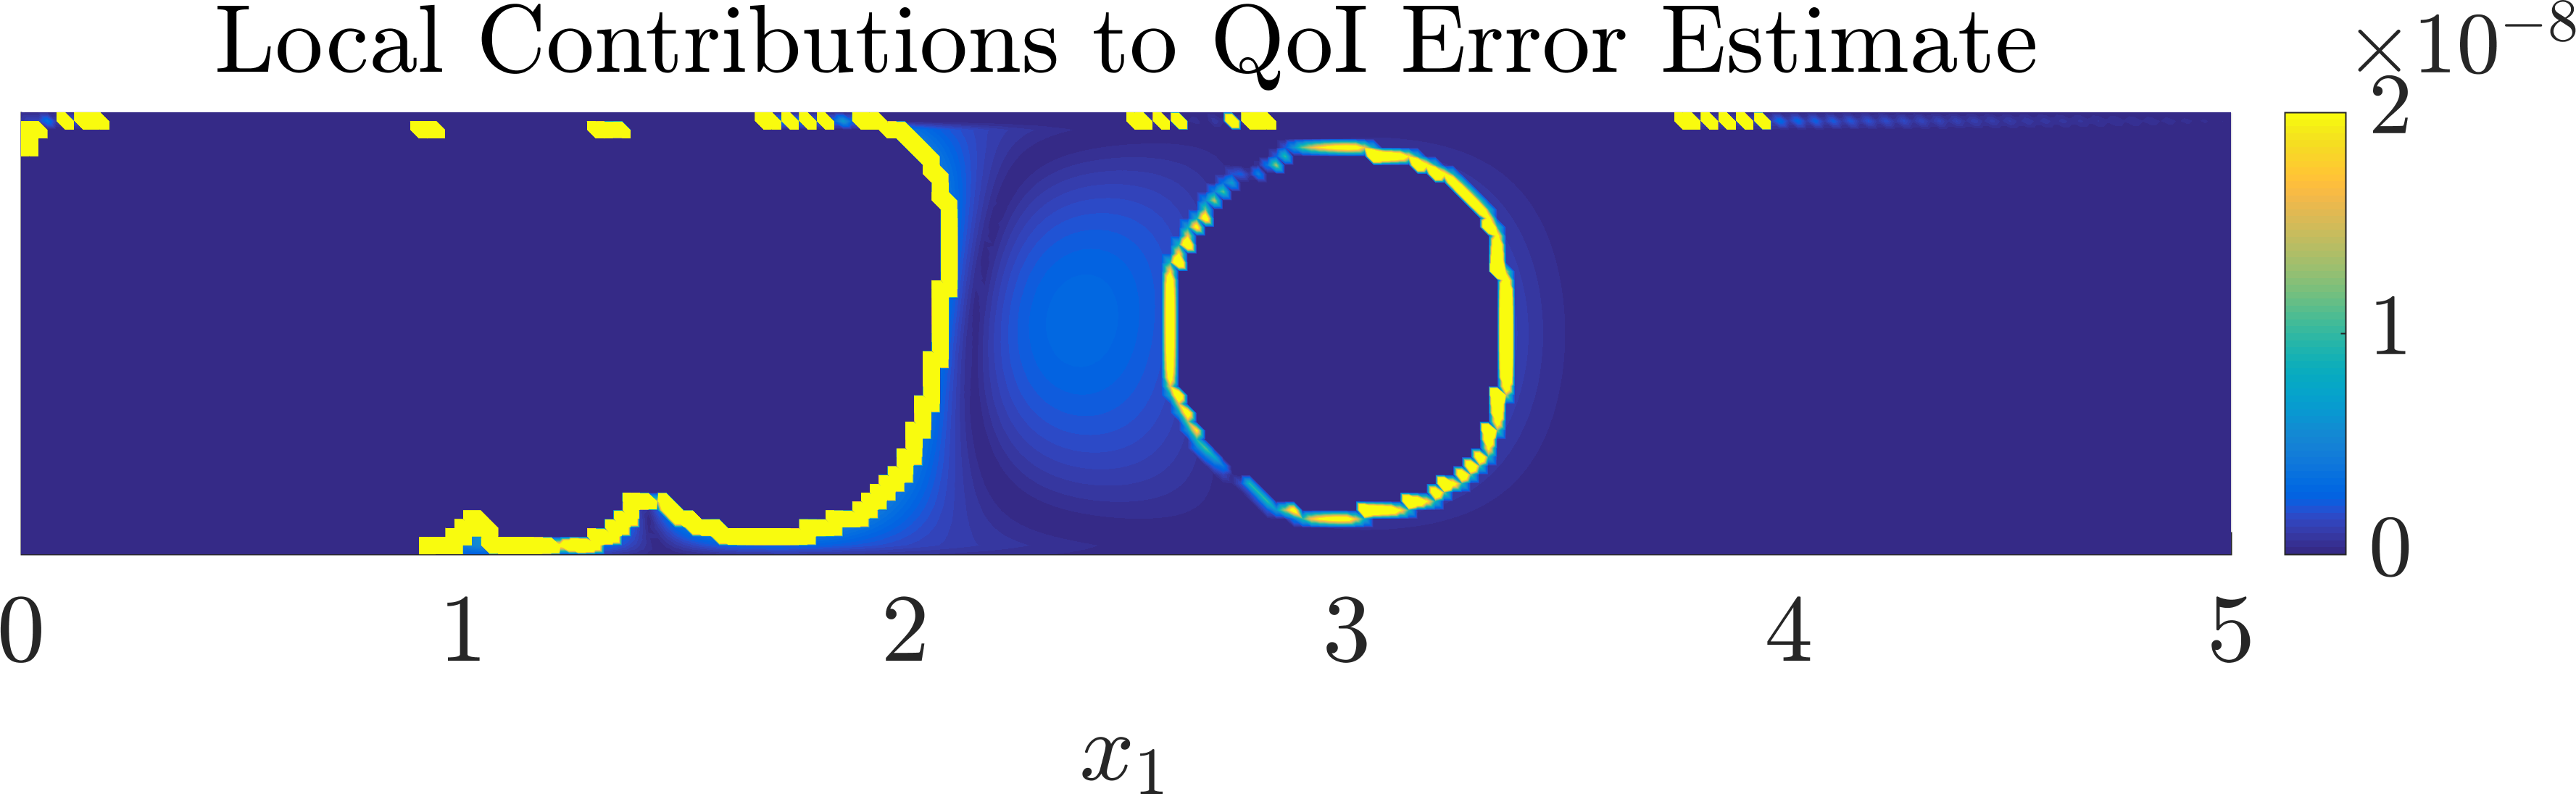
\includegraphics[width=0.51\textwidth]{svf/err_breakdown_MF05.png}
%  \vspace{-0.7\baselineskip}
%  \caption{MF$_5$ ($50\%$ HF)}
%  \vspace{0.8\baselineskip}
%\end{subfigure}
\subfloat[MF$_6$ ($60\%$ HF)]{
	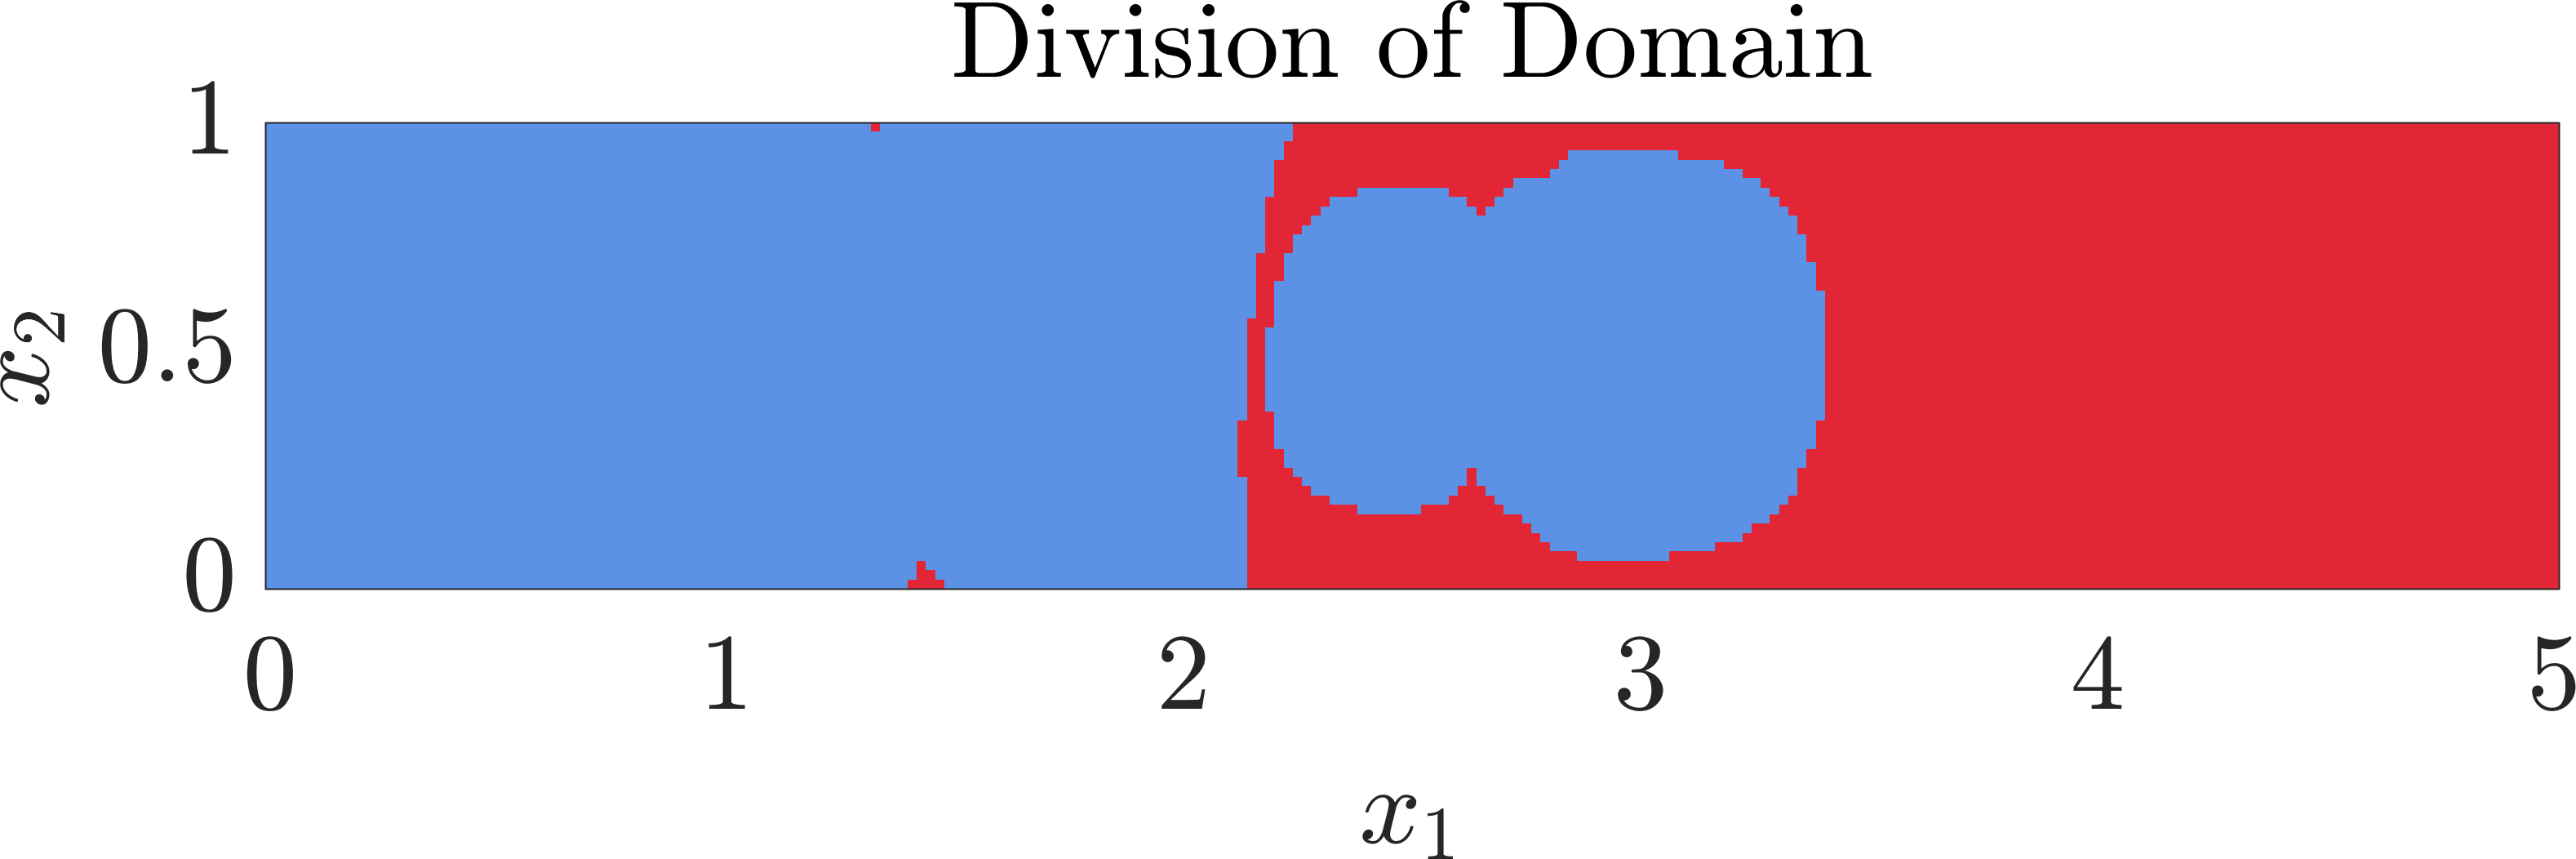
\includegraphics[width=0.46\textwidth]{svf/cd_cdr_MF06_divvy.png}
  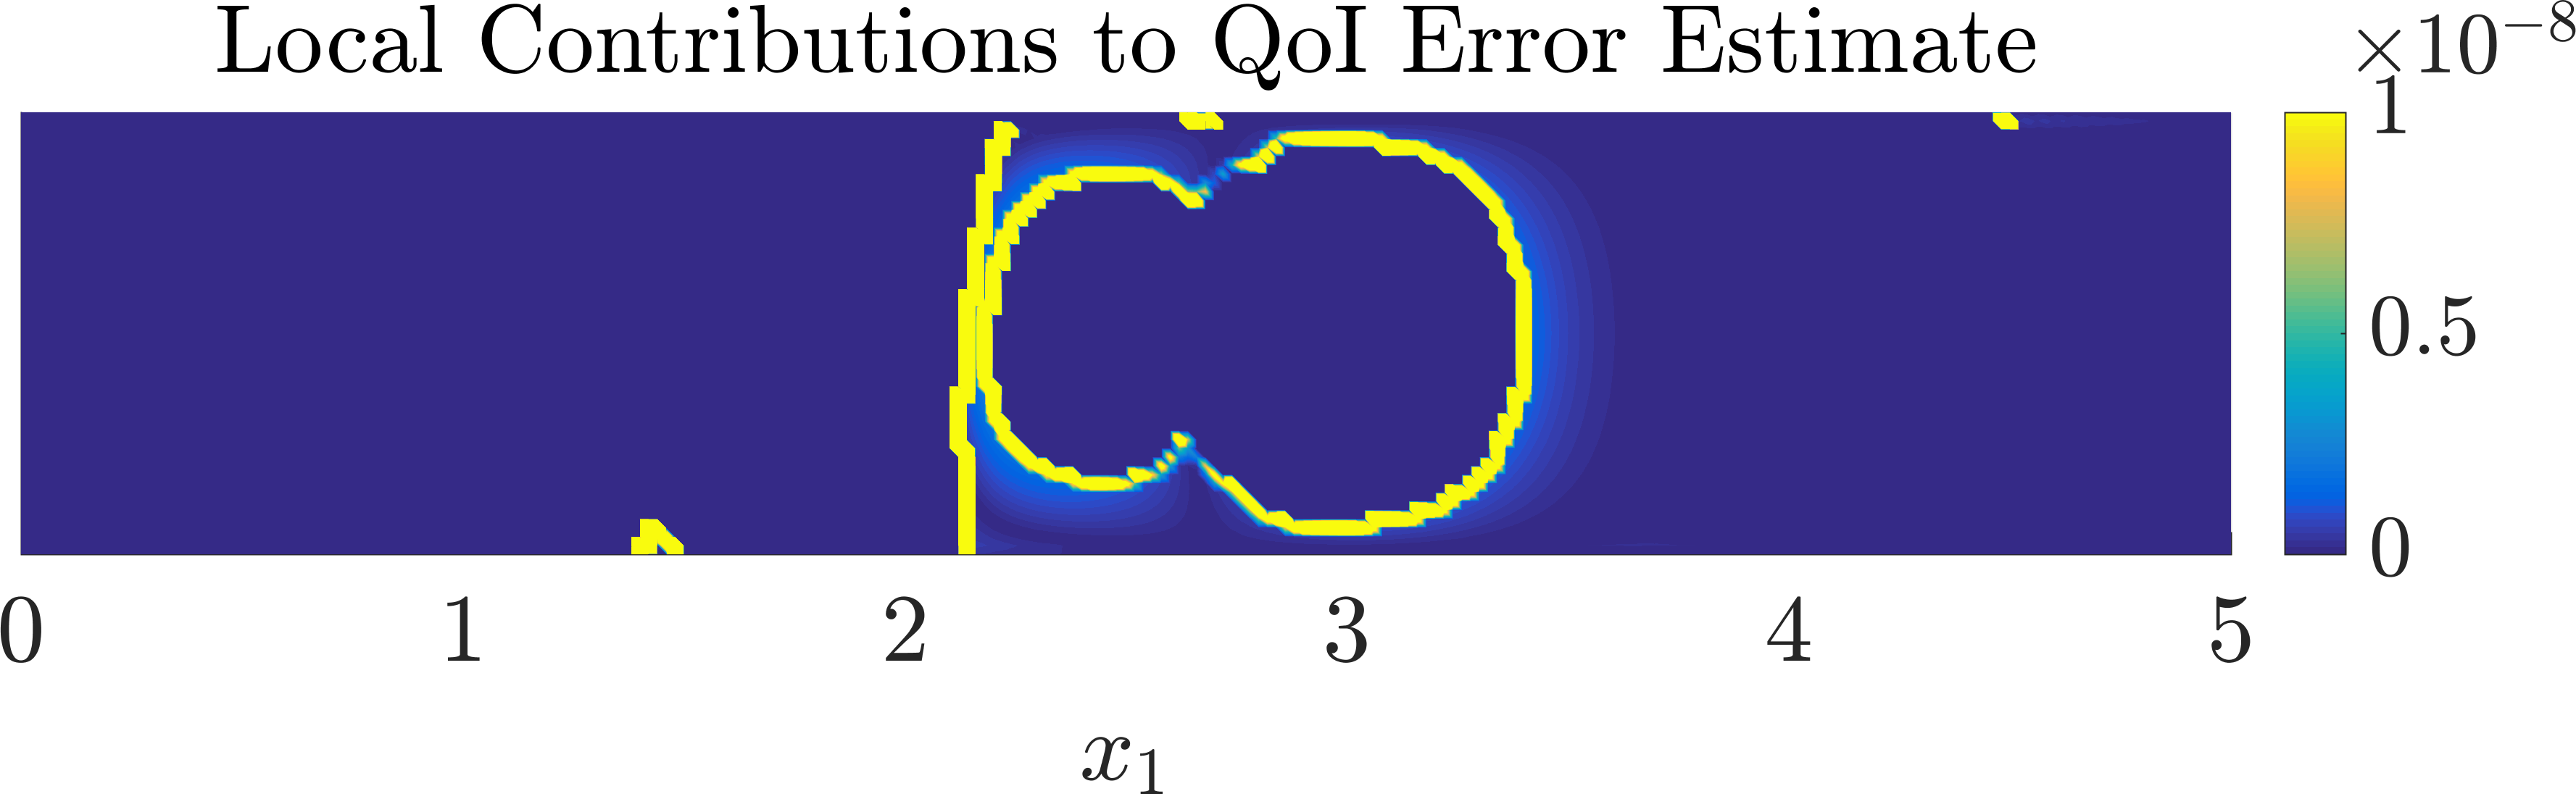
\includegraphics[width=0.49\textwidth]{svf/err_breakdown_MF06.png}
}
\caption{Left: Multi-fidelity refinement over the domain (low-fidelity constant-parameter model used in red portion, high-fidelity field-parameter model used in blue portion). Right: local error contributions. The (weighted) residual, and thus the local error contribution, tends to spike sharply at the interface between the low- and high-fidelity regions; the color range is truncated to make the error distribution visible elsewhere in the domain.}
\label{fig:svfRef}
\end{figure}
%
Comparing to \Cref{fig:baseRef}, we see that in this case the local error contribution is not as greatly concentrated around the QoI region and the nearest observation location; here, all three observation locations and the QoI region have associated regions of sufficiently similar high local error that all are refined in the first iteration. This reflects the global nature of the differences between the low- and high-fidelity models. 

The corresponding true and estimated absolute errors in the QoI are shown in \Cref{fig:svfErr}.
%
\begin{figure}[htbp]
\centering
\includegraphics[width=0.8\textwidth]{svf/err_est.pdf}
\caption{True and estimated absolute relative error in QoI, plotted as a function of the percentage area of the domain in which the high-fidelity field-parameter model is used.}
\label{fig:svfErr}
\end{figure}
%
In this case, we see that we must use the high-fidelity model in most of the domain in order to get an accurate QoI. The adaptive algorithm requires us to use the field representation of the high-fidelity model in much of the left half of the domain; this reflects the topology of the inferred parameter field in the high-fidelity inverse problem, which is only relatively constant towards the right portion of the domain. We also see that in this case, in contrast to the example in \Cref{sec:cdvcdrBaseRef}, increasing the proportion of the domain in which the high-fidelity model is used does not monotonically decrease the error in the QoI.

%------------------------------------------------------------------------------------------------------------------------%
\subsection{Combining Meshes and Physics in 3D} \label{sec:diffvcdr3D}
%------------------------------------------------------------------------------------------------------------------------%

In the previous examples, although the low- and high-fidelity models are sufficiently different to illustrate the behavior of \Cref{alg:refSeries}, they are both simple enough and similar enough that using \Cref{alg:refSeries} saves little, if any, computational effort. In this section, we consider a pair of models that differ in both the physics included and the mesh resolution, and we demonstrate computational savings using the multi-fidelity approach. In \Cref{sec:setup3D_diffmesh} we describe the setup of the models and their inverse problems, and in \Cref{sec:ref3D_diffmesh} we describe the results of applying \Cref{alg:refSeries} to this pair of models.

%------------------------------------------------------------%
\subsubsection{Problem Setup} \label{sec:setup3D_diffmesh}
%------------------------------------------------------------%

The two models share a box domain $\Omega(x_1,x_2,x_3)$ which is $2300$m, $1650$m, and $100$m long in the $x_1$, $x_2$, and $x_3$ directions, respectively. We will refer to the positive and negative directions in $x_1$ as ``east" and ``west", respectively. The high-fidelity model is a single-species convection-diffusion-reaction equation with a nonlinear reaction term, described by
%
\begin{subequations}
\label{eq:cdvcdrHF3D}
\begin{align}
\nabla\cdot(n\vec{V}u - nD\nabla u) + k_ru^2 = f(q) \quad &\text{in } \Omega, \label{eq:HFeq3D}\\
u = 0 \quad &\text{on } \partial \Omega_{west}, \\
\frac{\partial u}{\partial n} = 0 \quad &\text{on }\partial\Omega_{east}, \\
\hat{n}\cdot(n\vec{V}u - nD\nabla u) = 0 \quad &\text{on }\partial\Omega\backslash(\partial\Omega_{east}\cup\partial\Omega_{west}),
\end{align}
\end{subequations}
%
where the state $u$ is the mass-fraction (in parts-per-billion) of some contaminant species and $f(q)$ is a source/sink field. The velocity field is a constant $\vec{V}=(2.1,0,0)$ m/day. Given this velocity field and letting the molecular diffusion be negligible, we follow \cite{Vestedetal93} to express the (diagonal) dispersion tensor $D$ as $D_{11}=\alpha_{LH}V_1$, $D_{22}=\alpha_{TH}V_1$, and $D_{33}=\alpha_{TV}V_1$, where $\alpha_{LH}=100$m, $\alpha_{TH}=40$m, and $\alpha_{TV}=4$m are the longitudinal horizontal, transverse horizontal, and transverse vertical dispersivities, respectively; the dispersivity values were drawn from within the range of observed values in various porous media \cite{Davis86}. We have porosity $n=0.1$. The reaction coefficient is $k_r=4.2\cdot10^{-4}$ 1/day, chosen from within the wide range of reaction-rate coefficients for second-order reactions. Although the reaction term $k_ru^2$ does not correspond to any particular reaction of any particular species, we note that, in addition to second-order elementary reactions, a quadratic reaction term can appear in models of dissolution/precipitation processes in porous media \cite{Aha97} and biochemical degradation of petroleum hydrocarbons in soils \cite{Jack94}.

The low-fidelity model,
%
\begin{equation}
\nabla\cdot(- nk_d\nabla u) = f(q) \quad \text{in } \Omega, \label{eq:LFeq3D}
\end{equation}
%
differs in the removal of the reaction and convection terms and the anisotropy of the dispersion tensor; the dispersion tensor $D$ is replaced with a scalar $k_d=D_{11}$. The boundary conditions remain unchanged. As in the previous examples in \Cref{sec:cdvcdr}, the mixed-fidelity models are formed by dividing the domain into complementary subdomains $\Omega_{HF}$ and $\Omega_{LF}$, where \Cref{eq:HFeq3D,eq:LFeq3D} are solved, respectively. The QoI we wish to calculate is the integral of the state over a region $\Omega_I$.

The unknown parameters we wish to infer correspond to the source term $f(q)=q$; we impose $f(q)=q=0$ on the boundary $\partial\Omega$. Synthetic observations at 18 points in the domain are generated by running the high-fidelity model on a finer mesh. The locations of the observations as well as the QoI region $\Omega_I$ are shown in \Cref{fig:setup3D}. We set the regularization term in \Cref{eq:invOpt_obj} to be $R(q)=\frac{\beta}{2}\int_\Omega \|\nabla f(q)\|_2^2\:\textrm{d}V$.
%
\begin{figure}[htbp]
\centering
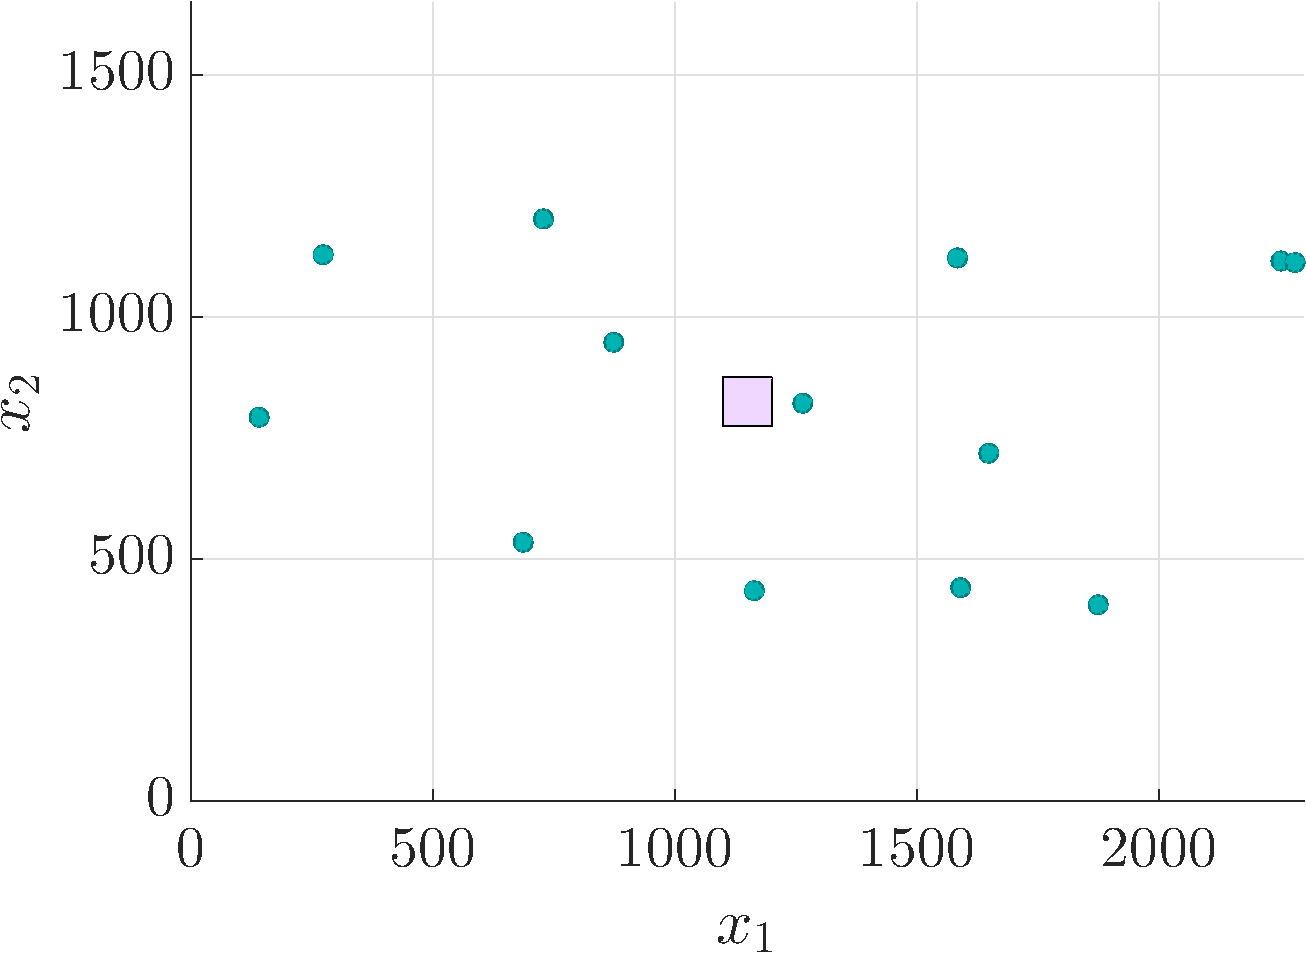
\includegraphics[width=0.4\textwidth]{series3D/setup_aerial_nolegend.pdf} \hfill
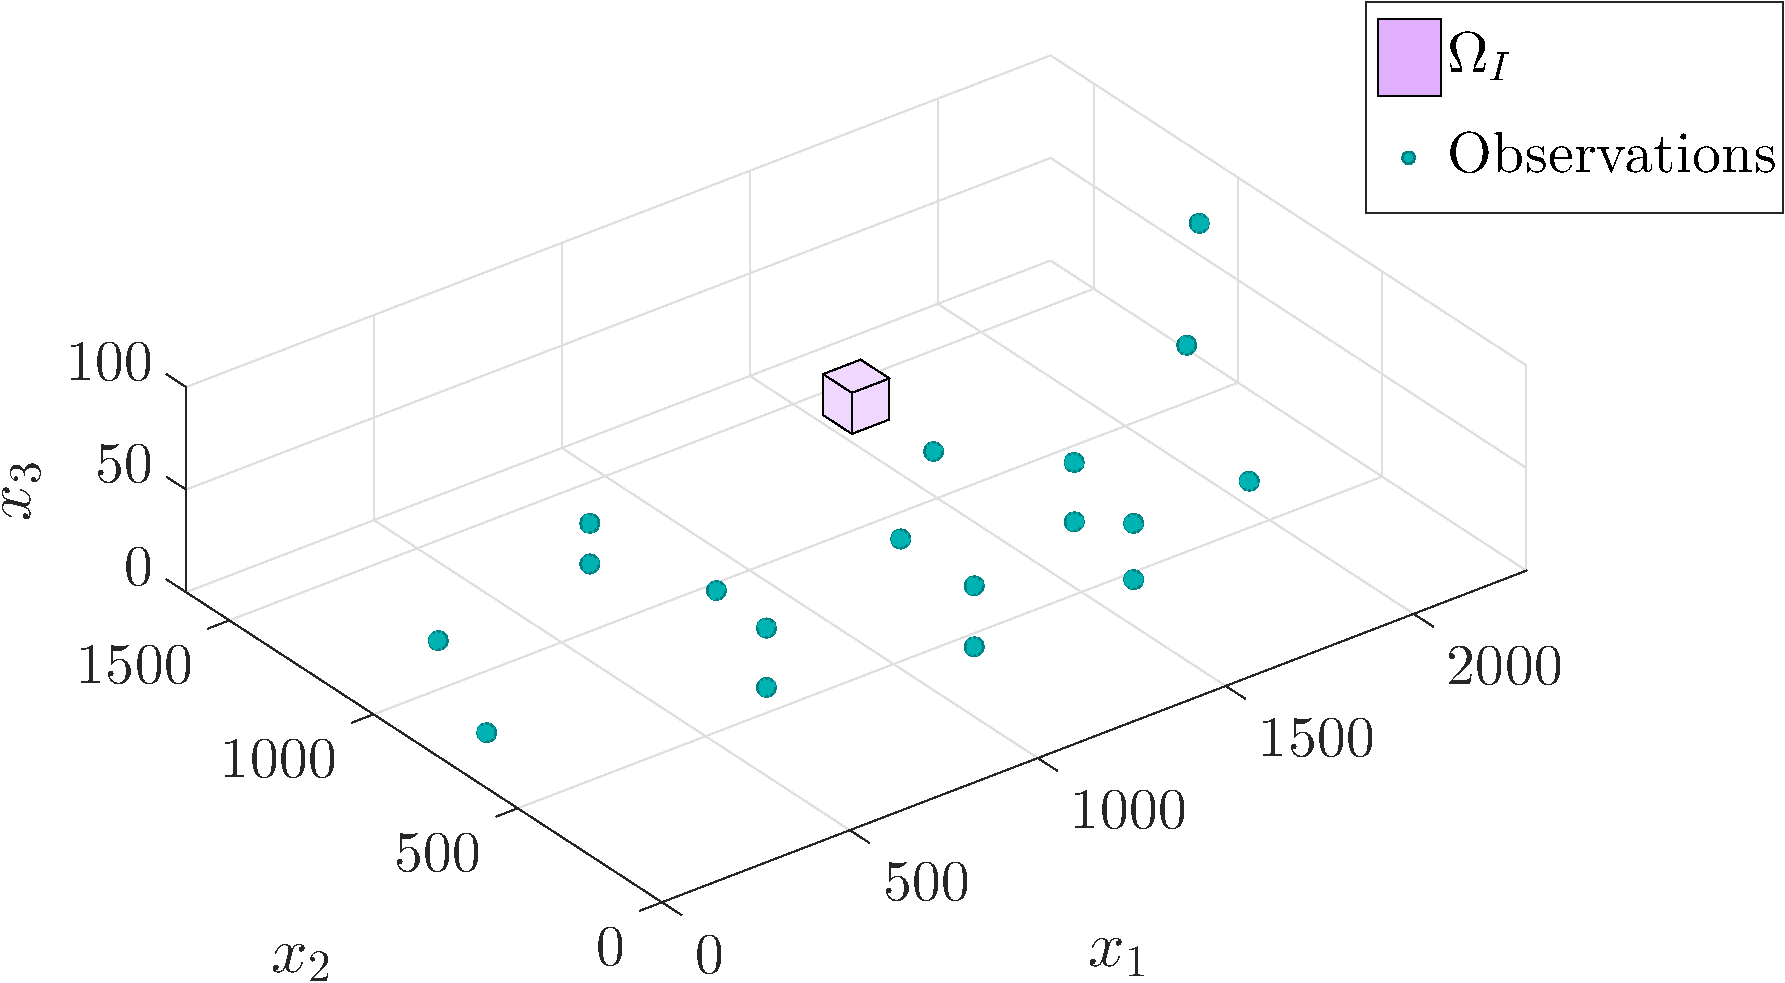
\includegraphics[width=0.55\textwidth]{series3D/setup_3view.pdf} \\
\vspace{\baselineskip}
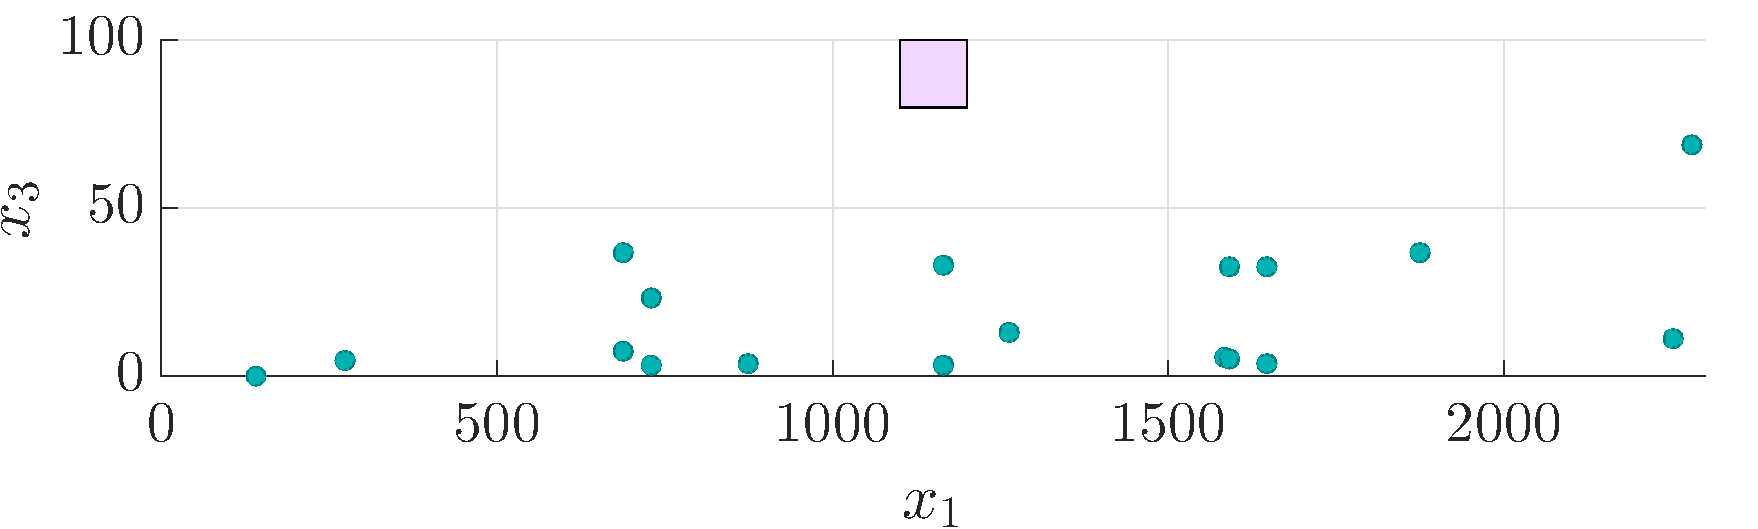
\includegraphics[width=0.6\textwidth]{series3D/setup_side_view.pdf}
\caption{Three views of the locations of the observations and the QoI region.}
\label{fig:setup3D}
\end{figure}
%

We use a FEM with a continuous Galerkin formulation and Lagrange elements. The lack of a convection term allows the low-fidelity model to be solved on a coarser mesh. For the high-fidelity model, the domain is discretized by 32, 64, and 32 elements along the $x_1$, $x_2$, and $x_3$ directions, respectively; for the low-fidelity model, the domain is discretized by 16, 32, and 16 elements along the $x_1$, $x_2$, and $x_3$ directions, respectively. The cell P\'{e}clet number is less than one and so stabilization is not required.

%------------------------------------------------------------%
\subsubsection{Adaptive Model Refinement Results} \label{sec:ref3D_diffmesh}
%------------------------------------------------------------%

We now present the results of solving the inference problem using \Cref{alg:refSeries}, with a relative error tolerance of $0.1\%$. At each iteration, we choose the $2\%$ of the basis functions with the largest error for model refinement; since each linear Lagrange basis function has eight elements in its support, the number of additional elements marked for refinement in each iteration is usually greater than for the 2D examples. All simulations are run on a single processor; we use the default nonlinear solver in \texttt{libMesh} \cite{libMeshPaper} (Newton's method with Brent line-search), and linear solves are performed using PETSc's \cite{petsc-user-ref} GMRES solver, preconditioned by incomplete factorization.

\Cref{tab:ref3D_diffmesh} shows the error at the end of each adaptive iteration. Each iteration of the adaptive algorithm uses the solution of the previous iteration as its initial guess. The number of degrees of freedom of each of the primary (and, if applicable, auxiliary) variables at each iteration is also given; the supplementary adjoint is solved on the high-fidelity mesh and thus each of its variables has the same number of degrees of freedom as each of the primary variables in the high-fidelity inverse problem. The high-fidelity inverse problem does not converge when the low-fidelity solution is used as an initial guess. Instead, we solve the inverse problem for an intermediate model
%
\begin{equation}
\nabla\cdot(n\vec{V}u - nD\nabla u) + k_ru^2 = f(q)
\end{equation}
%
and use the solution as an initial guess for the high-fidelity problem; equivalently, we use two steps of natural continuation on the reaction parameter: $k_r=0$, then $k_r=4.2\cdot10^{-4}$.
%
\begin{table}[htbp]
\caption{Runtime and relative errors of adaptive algorithm iterations given relative error tolerance of $0.1\%$; relative errors are given with respect to the high-fidelity QoI estimate.}
\label{tab:ref3D_diffmesh}
\centering
\begin{tabular}{|c|c|c|c|c|c|c|c|c|}
\hline
\multirow{2}{*}{Case} & \multirow{2}{*}{$\%$HF} & \multirow{2}{*}{DOFs} & \multirow{2}{*}{QoI} & Error & Error & $\%$ Relative \\
& & & & (Estimated) & (Actual) & Error (Actual)  \\ \hline
LF   & 0    & 9537  & 168710 & -16463 & -85663 & -103    \\
MF01 & 5.2  & 13417 & 167366 & -7207  & -84319 & -102    \\
MF02 & 11.4 & 17895 & 89777  & -6208  & -6730  & -8.10   \\
MF03 & 16.3 & 21001 & 85880  & -2473  & -2833  & -3.41   \\
MF04 & 22.0 & 24528 & 83902  & -711   & -855   & -1.03   \\
MF05 & 27.7 & 27984 & 83119  & 32     & -72    & -0.087  \\
HF   & 100  & 70785 & 83047  & --     & --     & --    \\ \hline
\end{tabular}
\end{table}
%

We notice that, compared to the results in \Cref{fig:baseErr}, the error estimates for the low-fidelity and first mixed-fidelity models are far from the true errors. This can be attributed to the linearization about $\Psi_{LF}$ and $\Psi_{MF_{1}}$ instead of $\Psi_{HF}$ in solving the supplementary adjoints as well as the third-order term that is ignored in the error estimate; the large differences in the QoI for the LF and MF01 models compared to the high-fidelity QoI indicate that $\Psi_{LF}$ and $\Psi_{MF_{1}}$ are significantly different from $\Psi_{HF}$. Compared to the pair of models in \Cref{sec:cdvcdrSetup}, the low- and high-fidelity models in this case are more dissimilar, even though in both \Cref{sec:cdvcdrSetup} and this case the nonlinear term in the high-fidelity model \Cref{eq:cdvcdrHF} and \Cref{eq:cdvcdrHF3D} is a quadratic reaction term. % KW: don't know what last part of this sentence means. what hi-fi models?
%The possibility of large inaccuracies in the error estimates of low-fidelity and mostly unrefined mixed-fidelity models suggests that one should use more than just the error estimate to decide when to stop the adaptive algorithm; a possible additional criterion could be to require that the estimated high-fidelity QoI ($I(q_{MF},u_{MF})+\epsilon_i$) for two consecutive iterations agree to within some tolerance. % KW: what behavior? this last sentence doesn't follow from the previous one. and what predicted hi-fi QOI? Do you mean mixed-fi? I'm not sure this is a good idea. I'd probably delete this last sentence.
% or just let the reader decide how to deal with possibly inaccurate initial error estimates?

The multi-fidelity domain refinements for the five adaptive iterations are shown in \Cref{fig:divvy3D_diffmesh}. Similarly to the behavior seen in \Cref{sec:cdvcdrBaseRef}, the QoI region and the areas around some of the measurement points are first targeted for refinement, with those measurement points furthest downstream of the QoI being the last to receive refinement. We also see that the domain is refined completely in the $x_3$ direction first around the QoI region, reflecting the large difference in the high-fidelity dispersion tensor $D$ and the low-fidelity dispersion coefficient in the $x_3$ direction.
%
\begin{figure}[htbp]
\centering
\subfloat[MF$_1$ ($5.2\%$ HF)]{
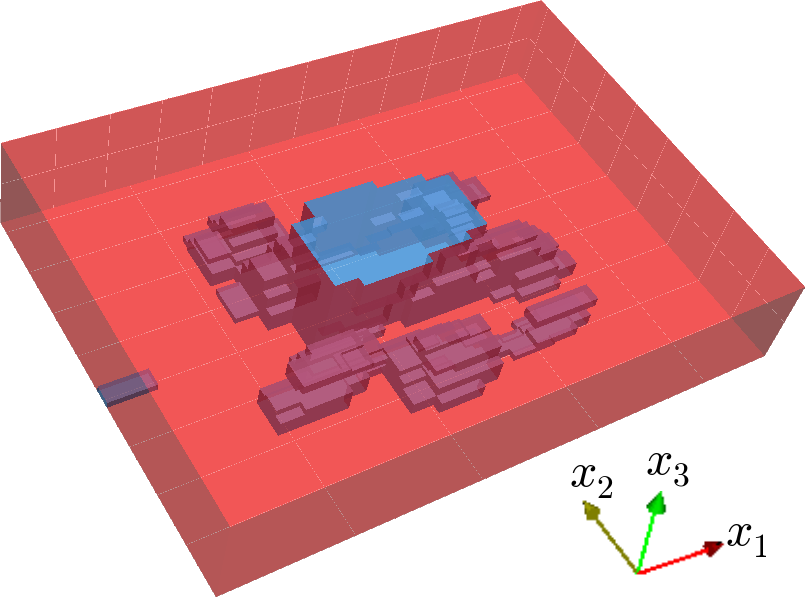
\includegraphics[width=0.31\textwidth]{series3D/run_diff_mesh/divvy1_whitebg_puff.png}
}
\subfloat[MF$_2$ ($11.4\%$ HF)]{
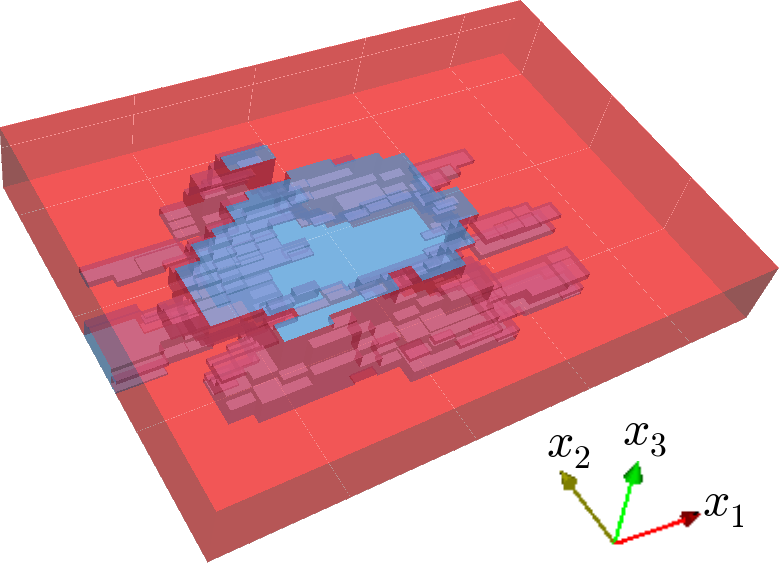
\includegraphics[width=0.31\textwidth]{series3D/run_diff_mesh/divvy2_whitebg_puff.png}
}
\subfloat[MF$_3$ ($16.3\%$ HF)]{
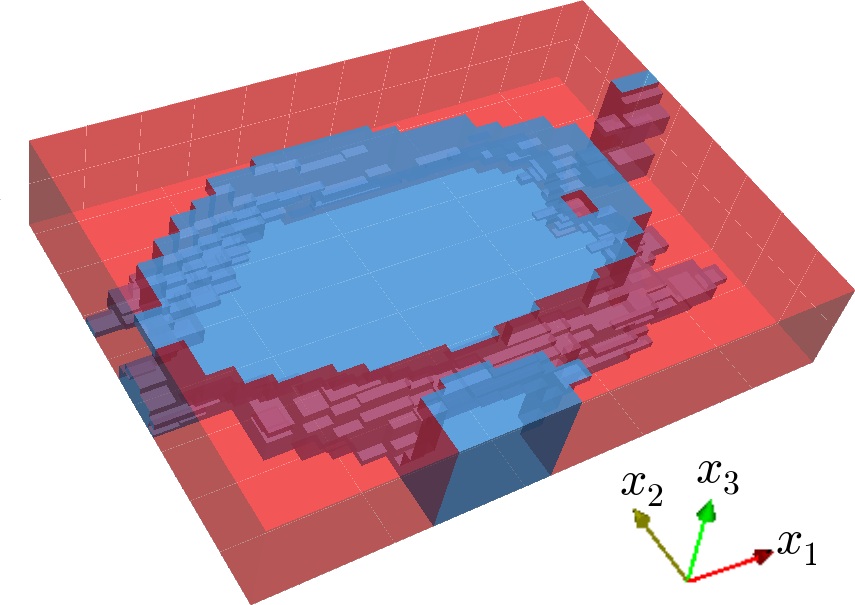
\includegraphics[width=0.31\textwidth]{series3D/run_diff_mesh/divvy3_whitebg_puff.png}
} \\
\subfloat[MF$_4$ ($22.0\%$ HF)]{
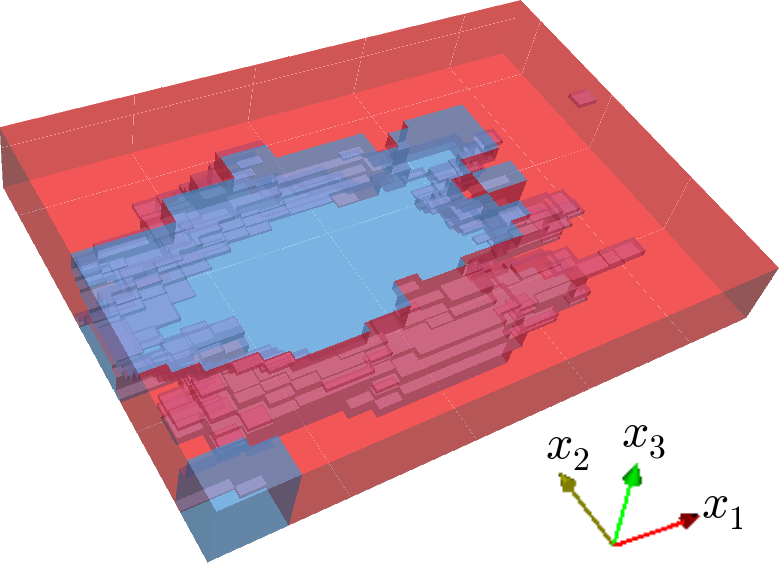
\includegraphics[width=0.31\textwidth]{series3D/run_diff_mesh/divvy4_whitebg_puff.png}
}
\subfloat[MF$_5$ ($27.7\%$ HF)]{
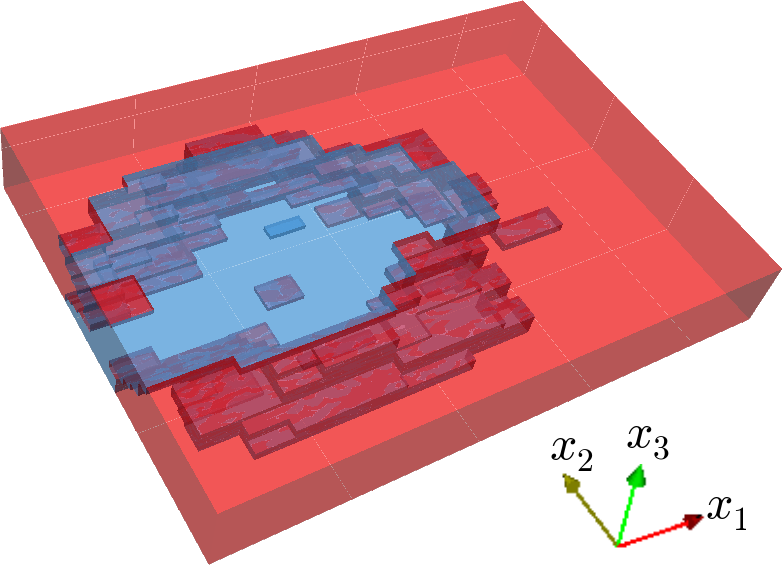
\includegraphics[width=0.31\textwidth]{series3D/run_diff_mesh/divvy5_whitebg_puff.png}
}
\caption{Domain division for mixed-fidelity models: low-fidelity convection-diffusion model used in red portion, high-fidelity convection-diffusion-reaction model used in blue portion (intermediate colors due to transparency indicate a mix of the two models along the line of sight); $x_3$ direction scaled for clarity.}
\label{fig:divvy3D_diffmesh}
\end{figure}
%

In this case, although the mixed-fidelity models have fewer degrees of freedom than the high-fidelity model, it is faster to solve the high-fidelity inverse problem than to adaptively seek a mixed-fidelity model with a small QoI error, starting from the low-fidelity model. This can be attributed to multiple factors: the high-fidelity problem is mildly nonlinear and has a close initial guess that is a solution to a linear system (when $k_r=0$), and the supplementary adjoint is solved on the high-fidelity mesh. Generally, as the nonlinearity of the high-fidelity model increases, one would expect solving the high-fidelity inverse problem to require more time relative to using the adaptive algorithm. However, one can also consider an ``offline-online" setting, where the mixed-fidelity models are identified up-front by applying \Cref{alg:refSeries} to a set of representative observations $d^*$. Then when actual/new data are received, one can solve the inverse problem with the mixed-fidelity model and the new data, and, if desired, compute an updated error estimate for the QoI. The mixed-fidelity inverse problems are expected to require less time to solve than the high-fidelity inverse problems.

To illustrate this offline-online application, we generate ten sets of noisy observations to represent the actual data gained during the online phase; the noisy observations are generated by taking the observations used in the adaptive algorithm and adding Gaussian white noise with standard deviation of $\sigma=0.02$ (equivalent to, on average, $5\%$ of the observed values). We then solve the inverse problem using each of the mixed-fidelity models depicted in \Cref{tab:ref3D_diffmesh,fig:divvy3D_diffmesh} as well as the high-fidelity model. The low-fidelity inverse problem is first solved and used as an initial guess for the higher-fidelity problems; we note that although there is a linear model that is more similar to the high-fidelity model than the low-fidelity model (i.e., convection-diffusion with anisotropic diffusivity and $k_r=0$ on the high-fidelity mesh) and thus would serve as a better initial guess, its existence is specific to our particular choice of models. The auxiliary and supplementary adjoint variables use a zero initial guess.

\Cref{tab:ref3D_newdata_QoI_diffmesh} shows the average QoI values, error estimates and solution times for the (non)linear solves. \Cref{tab:ref3D_newdata_times_diffmesh} shows the times needed to solve the inverse problems and to solve for the additional variables needed to obtain an error estimate. For six of the ten datasets, the high-fidelity inverse problem does not converge given the low-fidelity solution as an initial guess; these are solved using the $k_r=0$ solution as an initial guess so that true QoI errors can be calculated. The average high-fidelity inverse problem solution time shown in \Cref{tab:ref3D_newdata_times_diffmesh} includes only those cases (four of ten) that converged with the low-fidelity initial guess.
%
\begin{table}
\caption{Average QoI values and errors from solving inverse problem with mixed- and high-fidelity models and noisy data; relative errors are with respect to true high-fidelity QoI.}
\label{tab:ref3D_newdata_QoI_diffmesh}
\centering
\begin{tabular}{|c|c|c|c|c|c|}
\hline
\multirow{2}{*}{Case} & \multirow{2}{*}{$\%$HF} & \multirow{2}{*}{QoI} & Error & Error & $\%$ Relative  \\
& & & (Estimated) & (Actual) & Error (Actual) \\ \hline
LF   & 0    & 166774 & --    & -84326 & -102.3 \\
MF01 & 5.2  & 164597 & 4347  & -82149 & -99.65  \\
MF02 & 11.4 & 88867  & -5921 & -6418  & -7.79  \\
MF03 & 16.3 & 85237  & -2414 & -2789  & -3.38  \\
MF04 & 22.0 & 83411  & -724  & -963   & -1.17  \\
MF05 & 27.7 & 82664  & -18   & -216   & -0.26 \\
HF   & 100  & 82500  & --    & --     & --  \\ \hline
\end{tabular}
\end{table}

%
\begin{table}
\caption{Average times to solve inverse problem and obtain error estimate with mixed- and high-fidelity models and noisy datasets.}
\label{tab:ref3D_newdata_times_diffmesh}
\centering
\begin{tabular}{ccc|c|c|c}
\cline{4-5}
 & & & \multicolumn{2}{|c|}{Error Estimation} & \\
\cline{1-6}
\multicolumn{1}{|c|}{\multirow{3}{*}{Case}} & \multicolumn{1}{|c|}{\multirow{3}{*}{DOFs}} & Inverse & Auxiliary & Supplementary & \multicolumn{1}{|c|}{Total} \\
\multicolumn{1}{|c|}{} & \multicolumn{1}{|c|}{} & Problem & Variables & Adjoint & \multicolumn{1}{|c|}{Solution}\\
\multicolumn{1}{|c|}{} & \multicolumn{1}{|c|}{} & Time (s) &  Time (s) & Time (s) & \multicolumn{1}{|c|}{Time (s)}\\
\cline{1-6}
\multicolumn{1}{|c|}{LF}    & \multicolumn{1}{|c|}{9537}   & 16   & --  & -- & \multicolumn{1}{|c|}{--} \\ \hline
\multicolumn{1}{|c|}{MF01}  & \multicolumn{1}{|c|}{13147}  & 185  & 107 & 235 & \multicolumn{1}{|c|}{526} \\ \hline
\multicolumn{1}{|c|}{MF02}  & \multicolumn{1}{|c|}{17895}  & 328  & 169 & 206 & \multicolumn{1}{|c|}{703} \\ \hline
\multicolumn{1}{|c|}{MF03}  & \multicolumn{1}{|c|}{21001}  & 435  & 202 & 185 & \multicolumn{1}{|c|}{821} \\ \hline
\multicolumn{1}{|c|}{MF04}  & \multicolumn{1}{|c|}{24528}  & 406  & 201 & 188 & \multicolumn{1}{|c|}{795} \\ \hline
\multicolumn{1}{|c|}{MF05}  & \multicolumn{1}{|c|}{27984}  & 498  & 263 & 198 & \multicolumn{1}{|c|}{959} \\ \hline
\multicolumn{1}{|c|}{HF}    & \multicolumn{1}{|c|}{70785}  & 1185 & --  & --  & \multicolumn{1}{|c|}{1185} \\ \hline
\end{tabular}
\end{table}
%
We see that the mixed-fidelity models, when applied to noisy datasets different to those with which they were generated, continue to perform well in achieving a small error in the QoI while limiting the use of the high-fidelity model to less than a third of the domain. Given the same initial guess, the mixed-fidelity inverse problems takes less time on average than the high-fidelity inverse problem to solve, and they converge consistently.

